\documentclass[journal,twoside,web]{ieeecolor}
\usepackage{generic}
\usepackage{cite}
\usepackage{amsmath,amssymb,amsfonts}
\usepackage{algorithmic}
\usepackage{graphicx}
\usepackage{textcomp}
\def\BibTeX{{\rm B\kern-.05em{\sc i\kern-.025em b}\kern-.08em
    T\kern-.1667em\lower.7ex\hbox{E}\kern-.125emX}}
\markboth{\journalname, VOL. XX, NO. XX, XXXX 2023}
{Author \MakeLowercase{\textit{et al.}}: Short Wave Infrared Neuromodulation Gadget (May 2023)}
\begin{document}
\title{Short Wave Infrared Neuromodulation Gadget (May 2023)}
\author{Cameron R. Author, \IEEEmembership{Member, IEEE}, Matthew T. Author, Bibhus L. Author, 
        Krishna S. Sponsor, \IEEEmembership{Member, IEEE}, John L. Mentor, \IEEEmembership{Member, IEEE}
\thanks{ }
\thanks{ }
\thanks{ }
\thanks{ }}

\maketitle

\begin{abstract}
Direct stimulation of neurons in the brain can potentially treat many diseases, such as Parkinson's 
or Alzheimer's disease. Direct stimulation, whether it be through electric or photonic stimulation, 
provided a way to activate neurons in the brain and treat diseases and conditions. However, this kind 
of invasive stimulation can have risks that lead to worsening the condition or cause infection. 
The Short-Wave Infrared Neuromodulation Gadget (SWING) aimed to build and test a non-invasive optical method 
of stimulation with funding provided by the KIND laboratory's Brain IMPACT project. SWING is part of the 
two semester long Electrical and Computer Engineering capstone sequence. The first semester was focused on research 
and design, and the second semester is focused on prototyping and testing.

Three components were used to accomplish SWING's goal of non-invasive stimulation: a 1550 nanometer (nm) laser, 
an Optical Phantom human head, and simulation software. The 1550 nm laser acted as the stimulating source, 
aiming to provide optical energy to the phantom and activate neurons. Without clinical trials, SWING implemented an epoxy resin 
Optical Phantom with different concentrations of absorbing and scattering agents and approximating the layers of the human head's 
optical properties. Because the optical coefficients of biological tissue are not well known at 1550 nm, 
SWING used a cubic extrapolation to approximate these coefficients. Monte Carlo eXtreme (MCX) was then used to predict the 
expected photon distribution and intensity throughout a model of the human head. Experimentally, the intensity was investigated 
based on its correlation to neuron activity. Using the simulation and laser setup, the results compared the simulated values to the 
experimentally acquired values. This information provided a basis on the validity of using a 1550 nm neuromodulation device to treat 
diseases and conditions.
\end{abstract}

\begin{IEEEkeywords}

\end{IEEEkeywords}

\section{Introduction}
\label{sec:introduction}
There are many physical issues in the brain, including Parkinson's disease and functional problems such as attention-deficit/hyperactivity disorder (ADHD) 
and depressive disorders. A solution to such problems that has been explored recently in the Neurotech community is one that involves a direct stimulation of 
neuronal connections in the brain [1]. Direct neuronal stimulation, whether it be through electric or photonic stimulation, provides a way to control 
mechanisms in the brain and treat diseases and conditions. These treatments result in an improvement of the effects caused by these diseases and conditions. 
However, most modern neuromodulation strategies are invasive in nature, and there are limited options for a non-invasive approach to neuromodulation for medical benefit. 
Many invasive techniques involve surgical implants and increase the risk of brain hemorrhage and worsening mental and emotional status for some patients, 
that often make the cons worse for life-threatening conditions [1]. As a result, SWING looks to create a non-invasive method for neuromodulation 
using a near-infrared photonic stimulation method.

SWING is sponsored by Dr. Krishna and mentored by Dr. Ziaeefard from the Ohio State University Department of Electrical and Computer Engineering and is additionally mentored by 
Dr. LaRocco from the Ohio State University Wexner Medical Center. The stakeholders for this project are researchers, doctors, medical professionals, 
as well as both inpatients and outpatients. The needs for this project make up the following categories: safety, performance, user-friendly, non-invasive, wearable, and realistic. 
To ensure that each portion of SWING meets these needs, each need is assigned a requirement discussed later in this report.

Solving the problems previously discussed has the potential to reduce the effects of brain disorders on the general population, leading to overall improvement of health. 
This solution can also mitigate the risks of surgery that patients would have to go through if done invasively, again improving public health.

\section{Methods}
\label{sec:methods}

\section{Results}
\label{sec:results}

\begin{figure}[!htb]
    \center{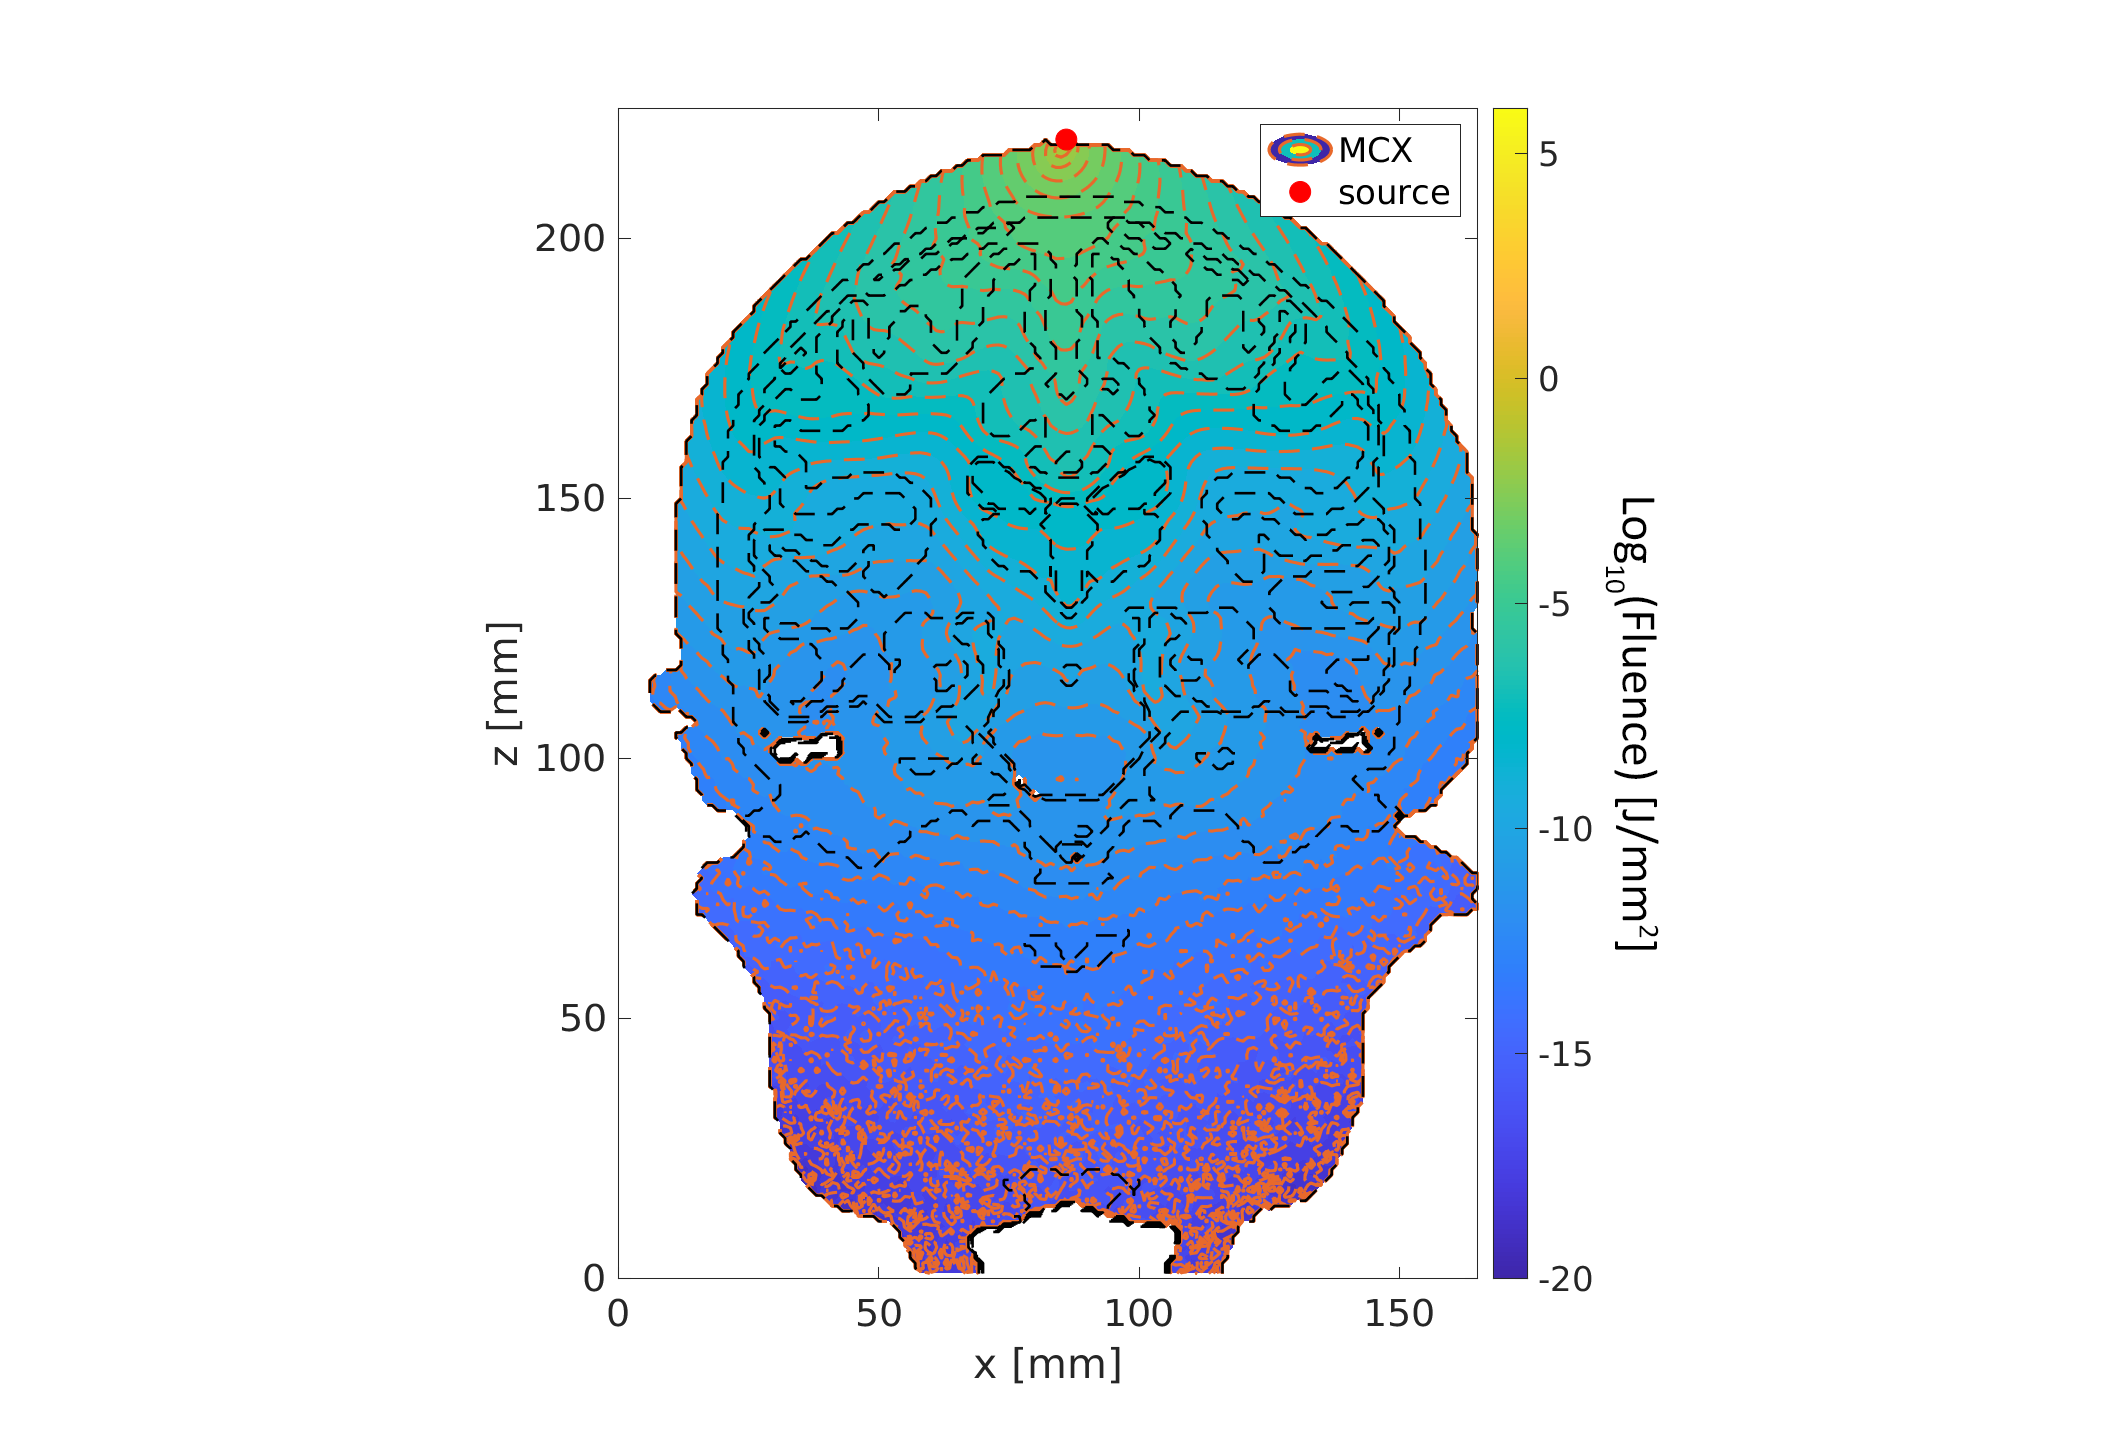
\includegraphics[width=\columnwidth]
    {Figures/Fluence_Distribution_810nm_CZ.png}}
    \caption{\label{fig:810-CZ} 810 nm CZ Position}
\end{figure}

\begin{figure}[!htb]
    \center{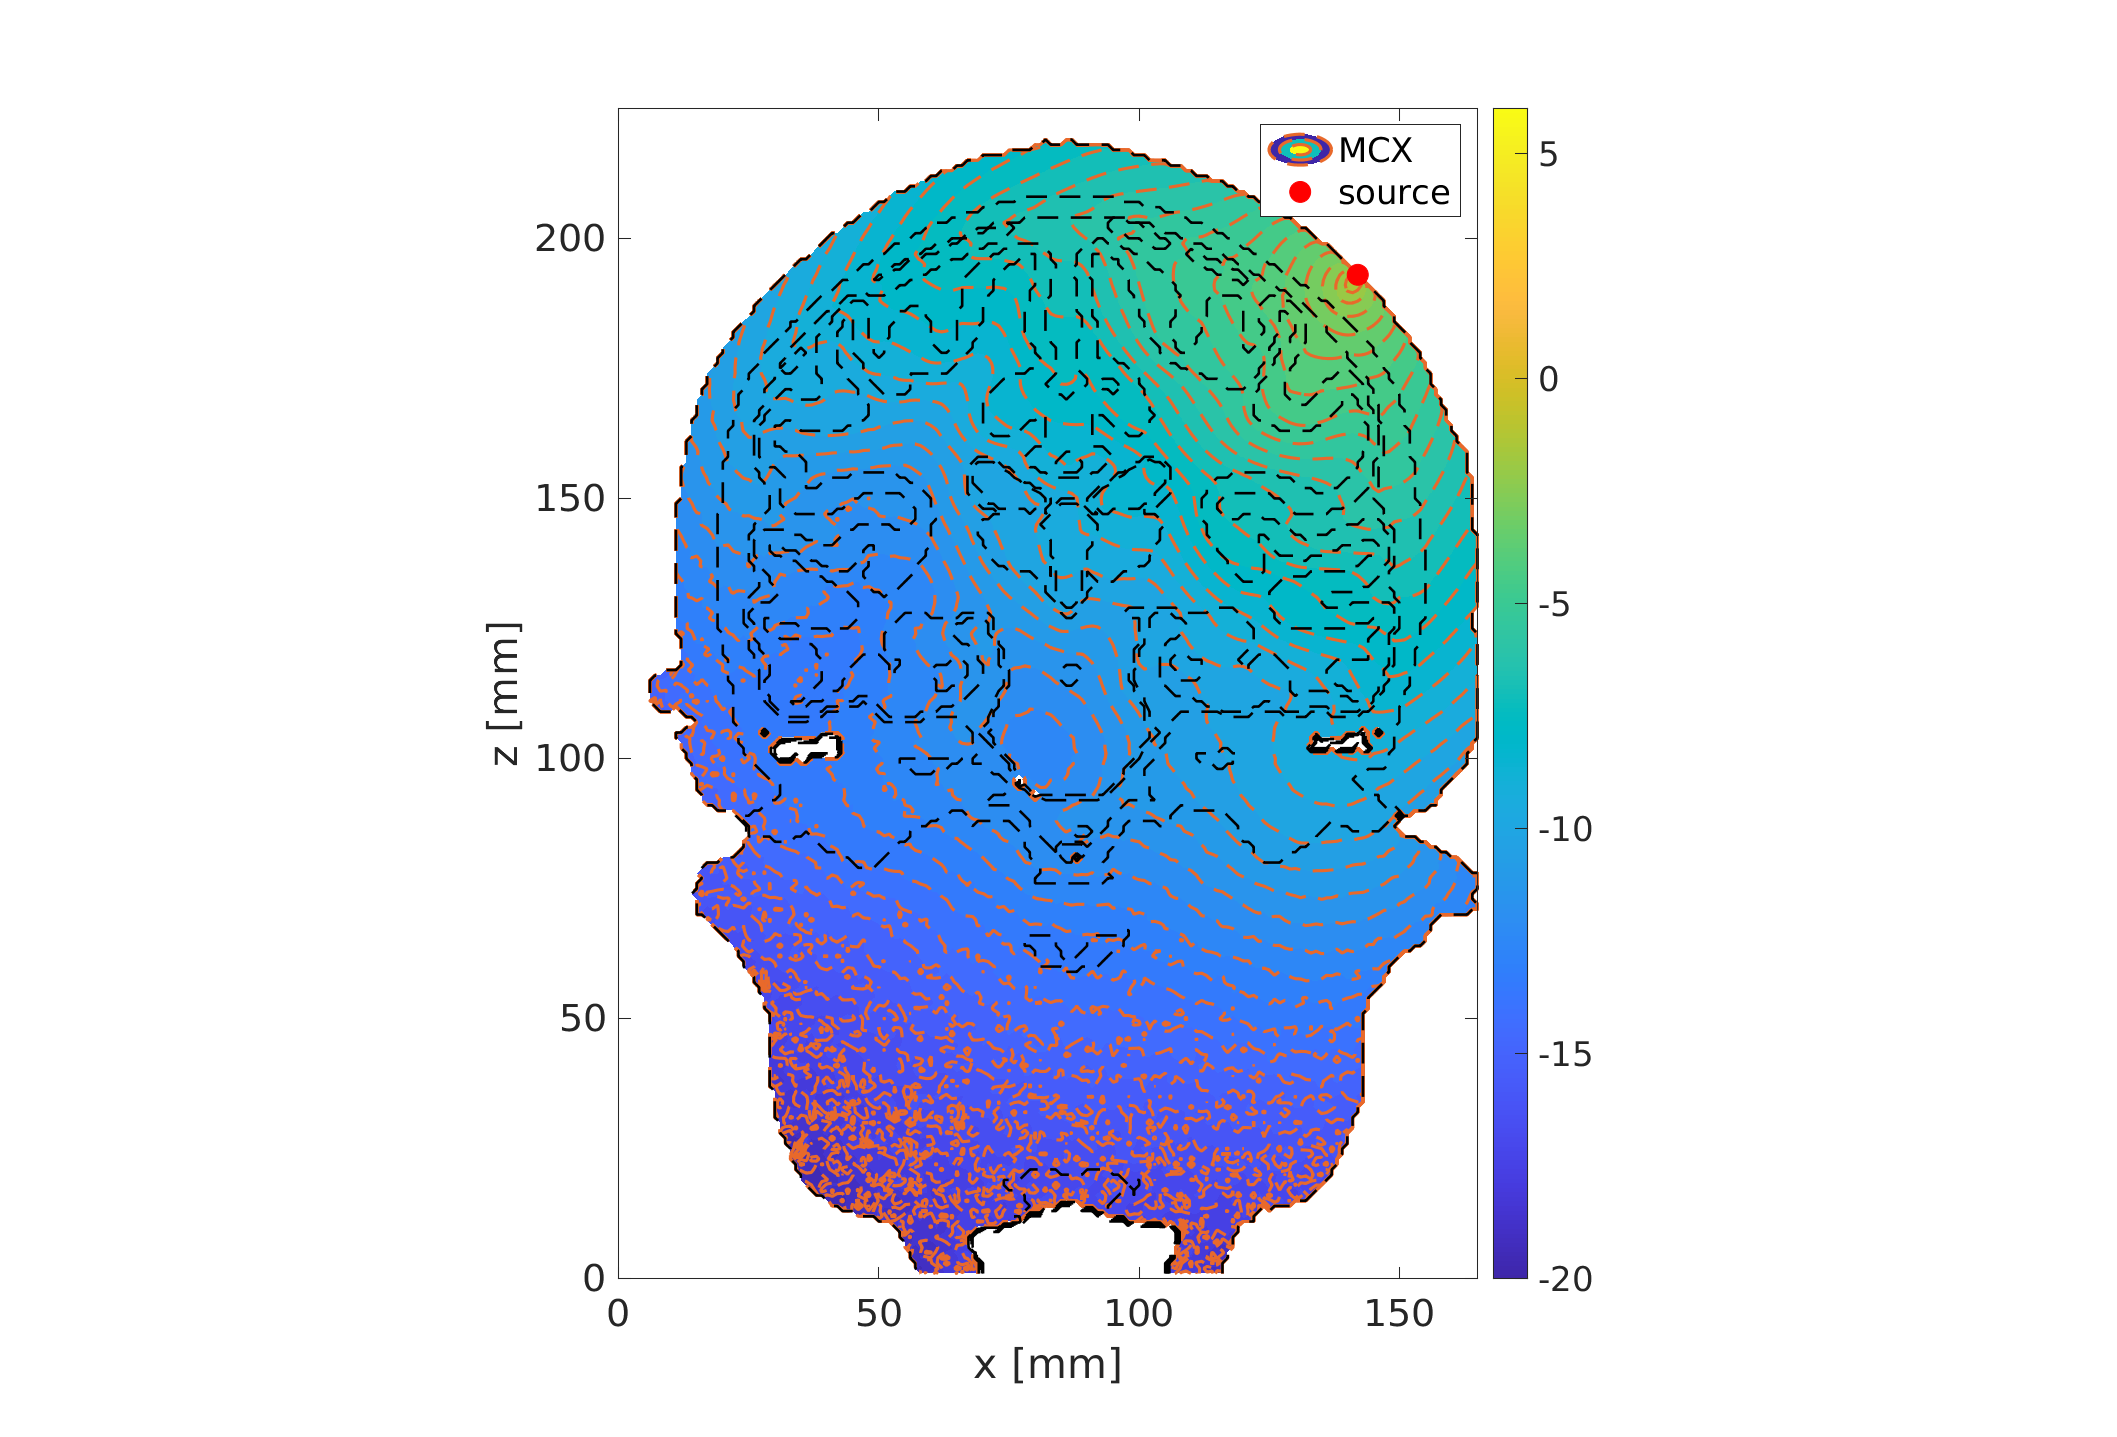
\includegraphics[width=\columnwidth]
    {Figures/Fluence_Distribution_810nm_45deg.png}}
    \caption{\label{fig:810-45} 810 nm 45 Degree Position}
\end{figure}

\begin{figure}[!htb]
    \center{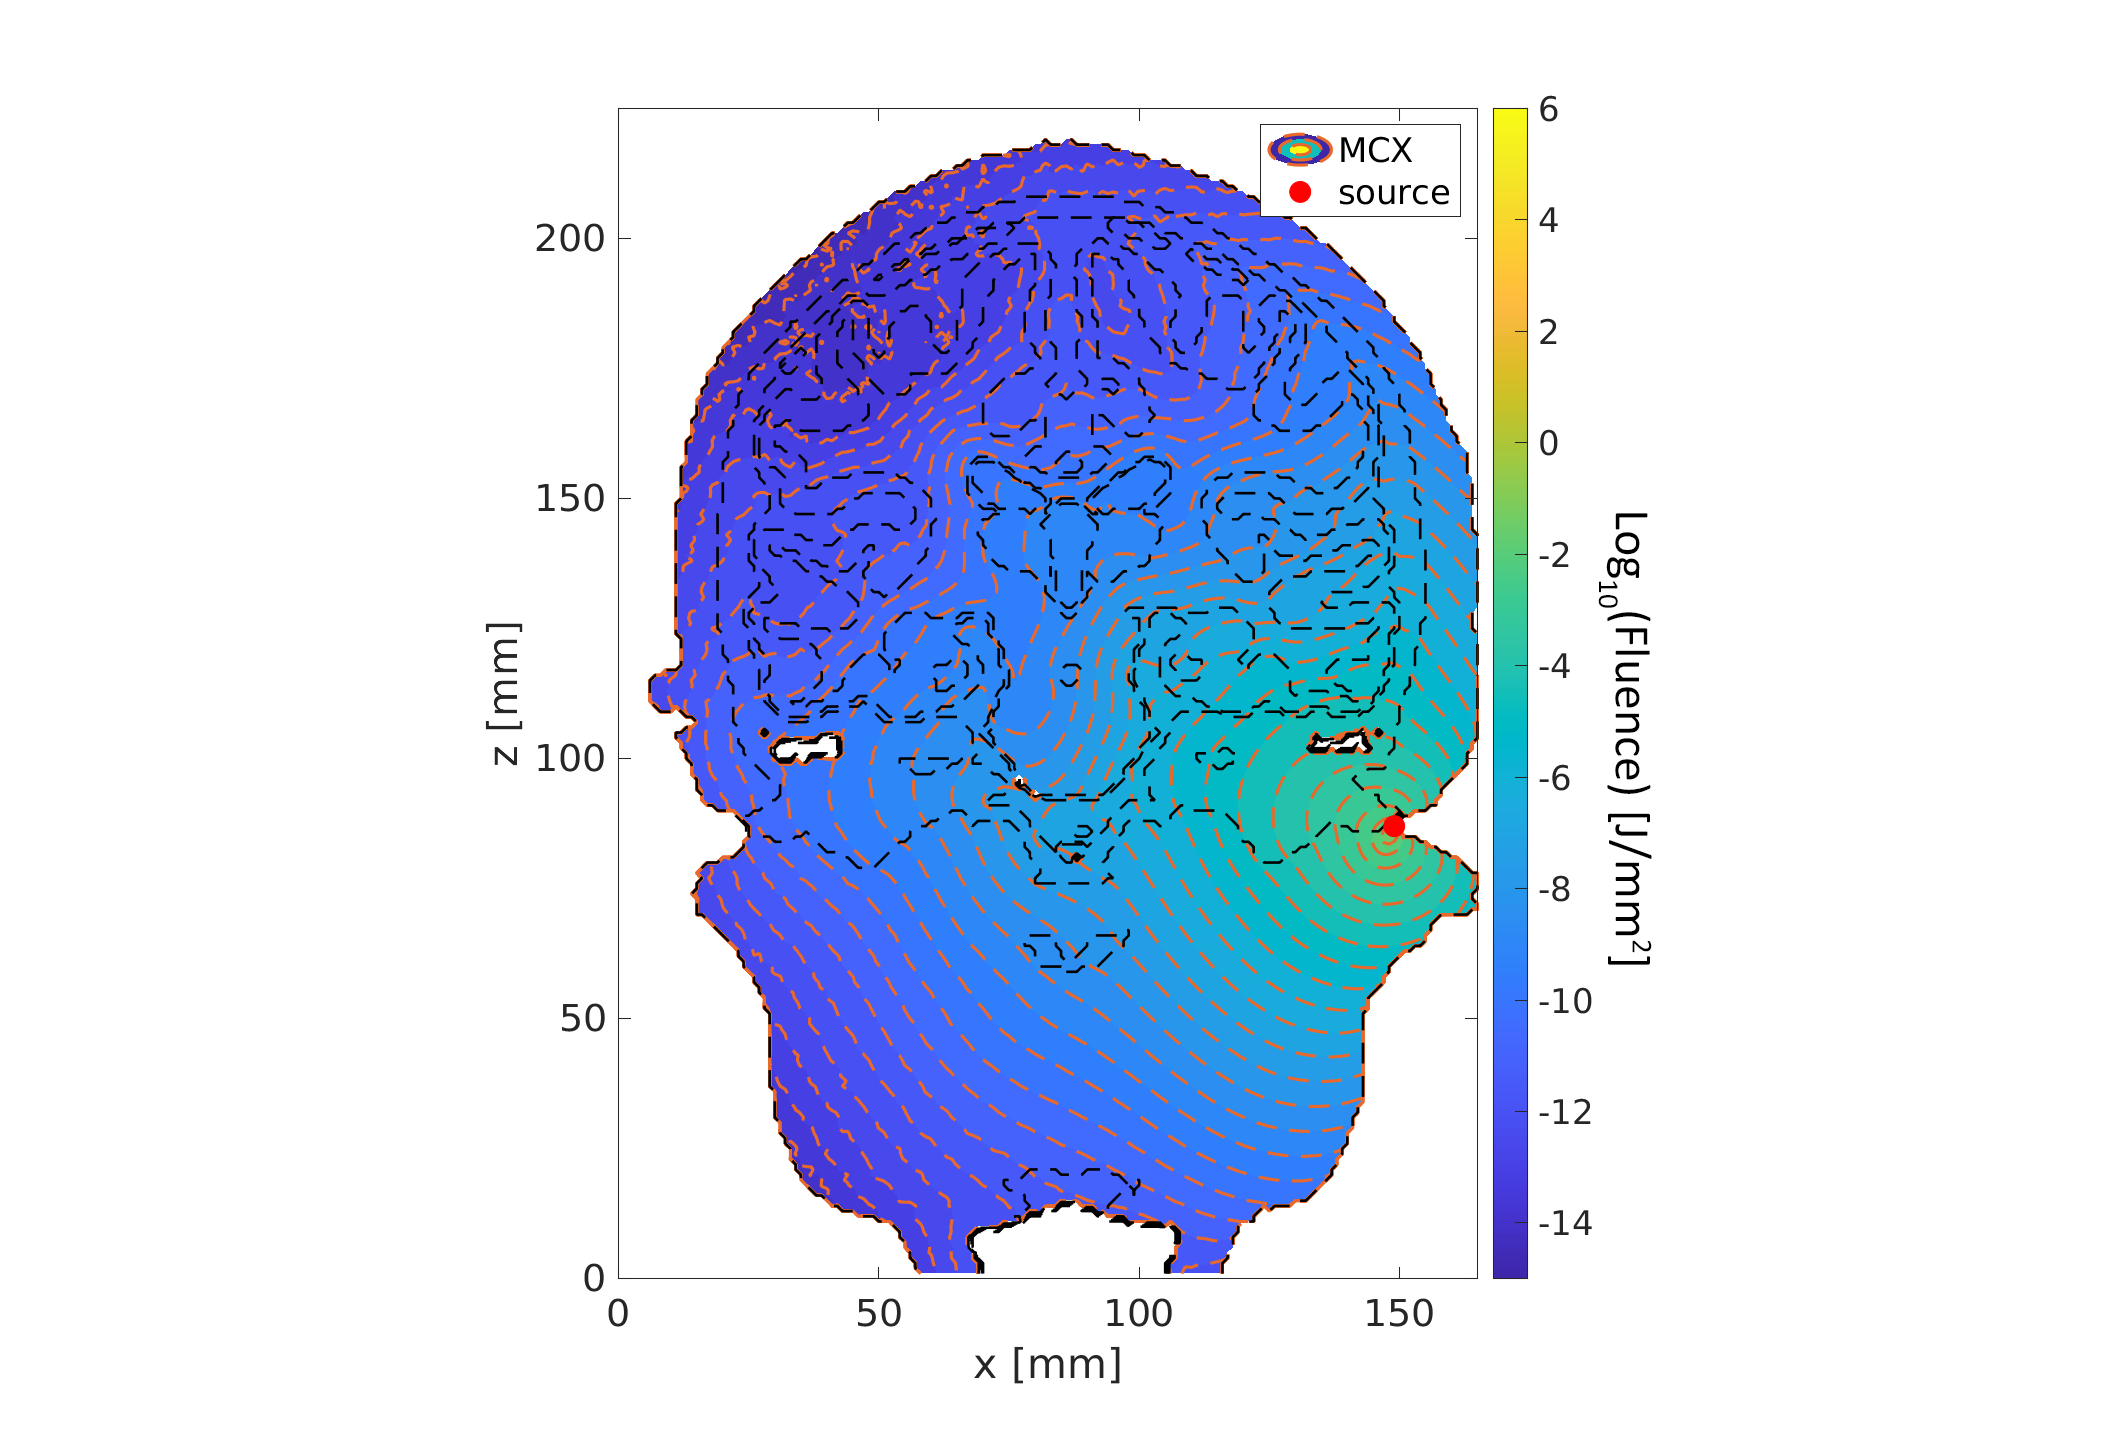
\includegraphics[width=\columnwidth]
    {Figures/Fluence_Distribution_810nm_Cochlear.png}}
    \caption{\label{fig:810-Cochlear} 810 nm Cochlear Position}
\end{figure}

\begin{figure}[!htb]
    \center{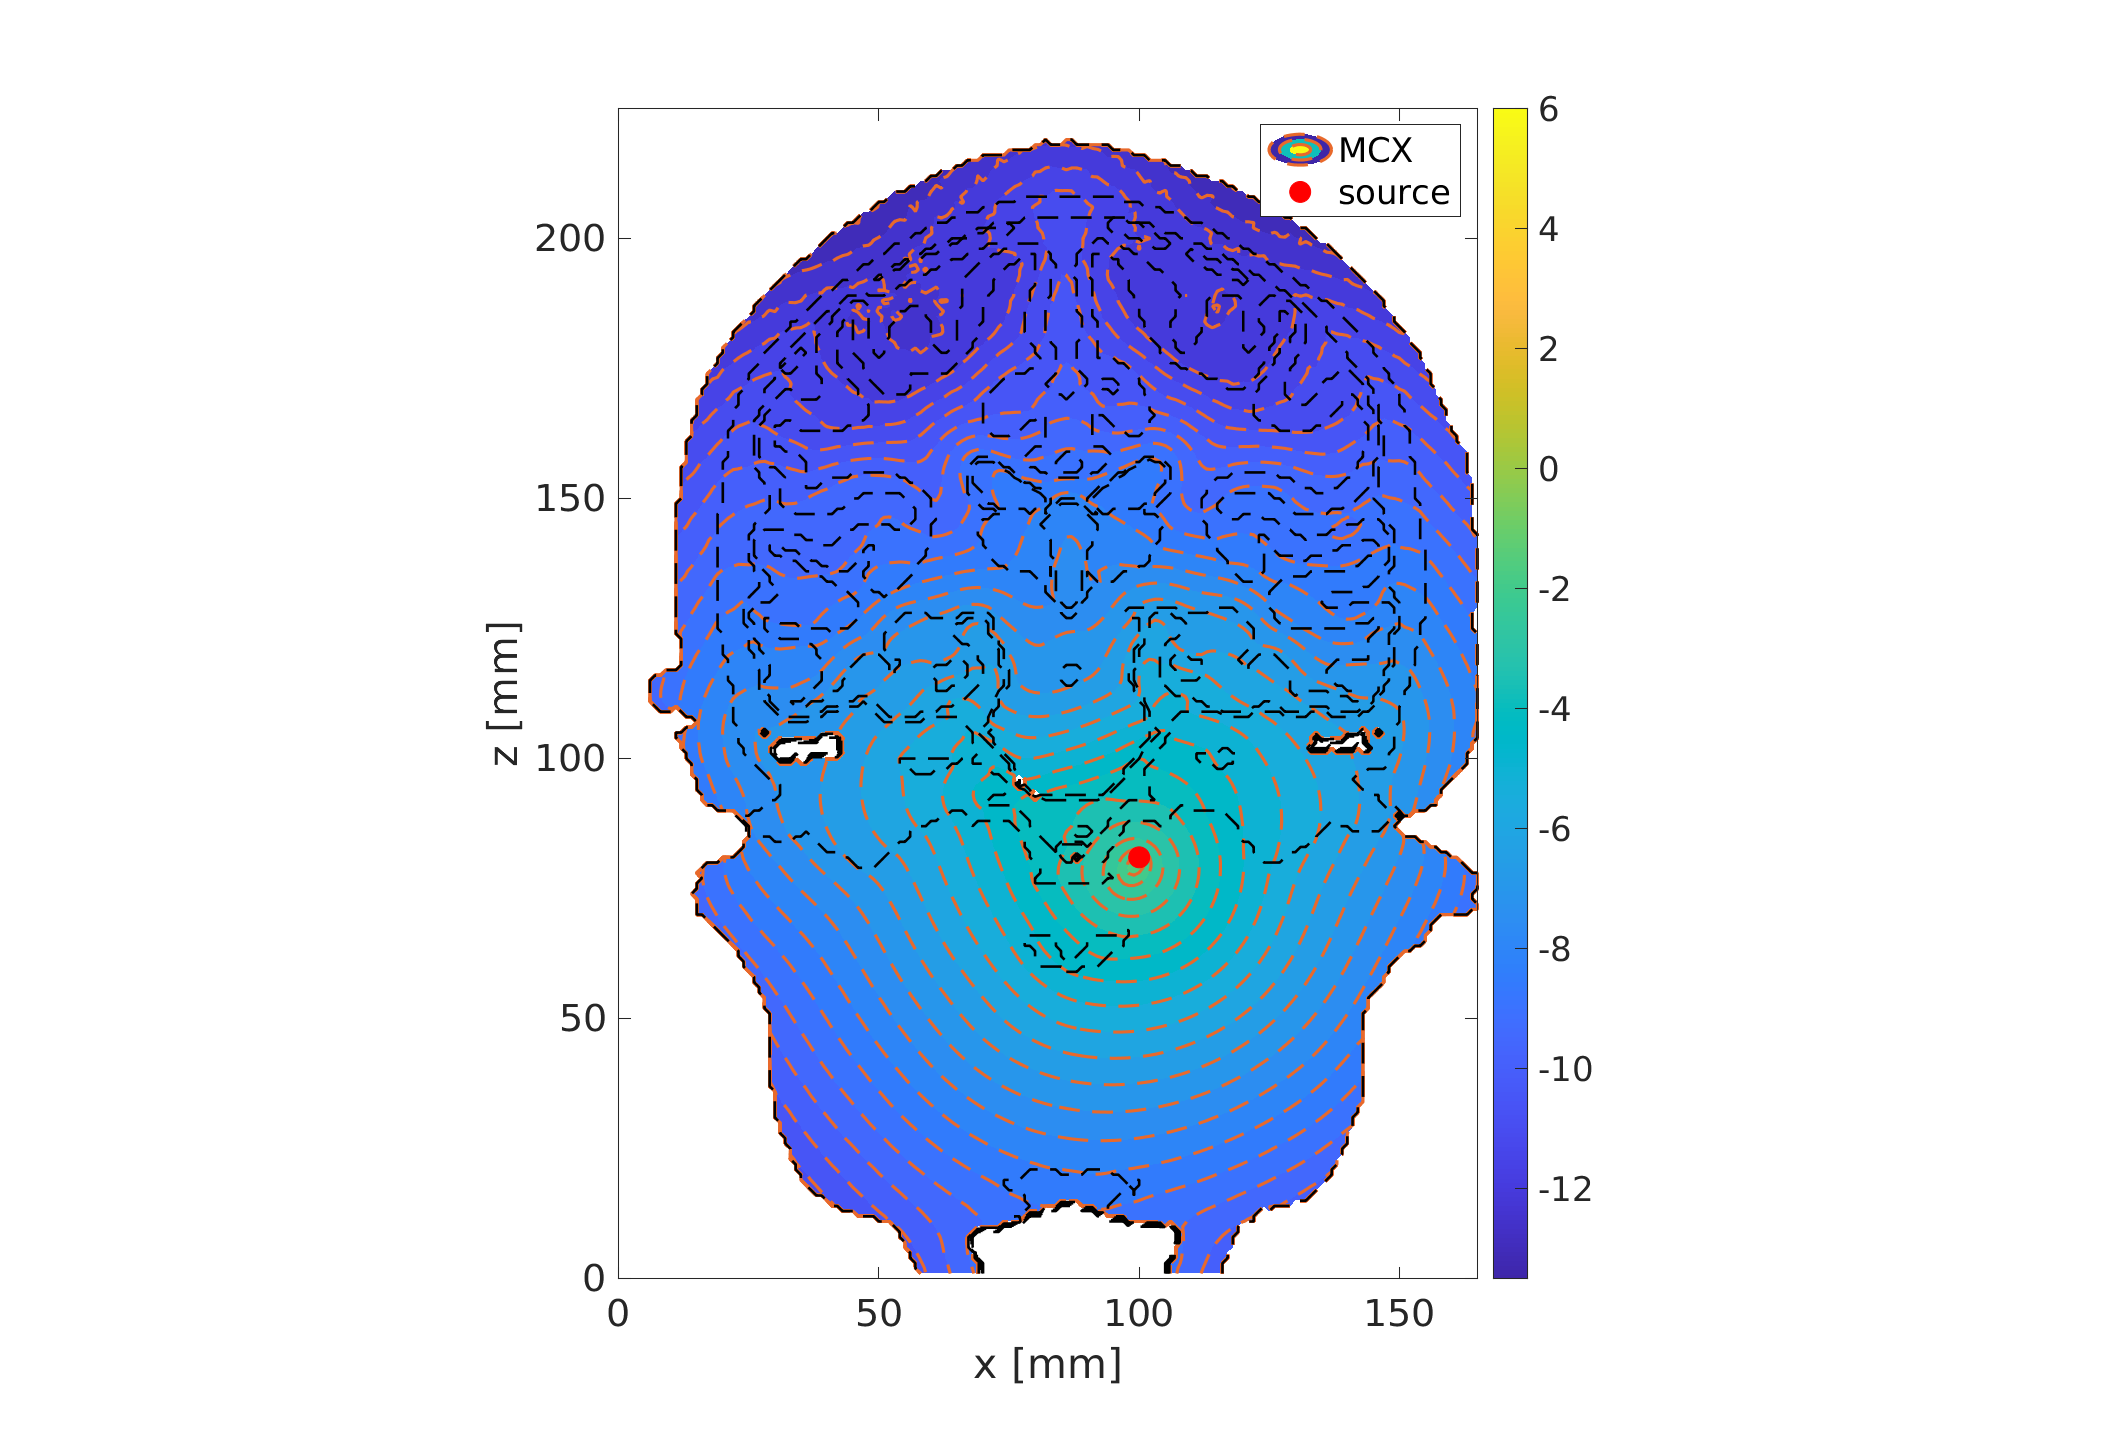
\includegraphics[width=\columnwidth]
    {Figures/Fluence_Distribution_810nm_Intranasal.png}}
    \caption{\label{fig:810-Intra} 810 nm Intranasal Position}
\end{figure}

\begin{figure}[!htb]
    \center{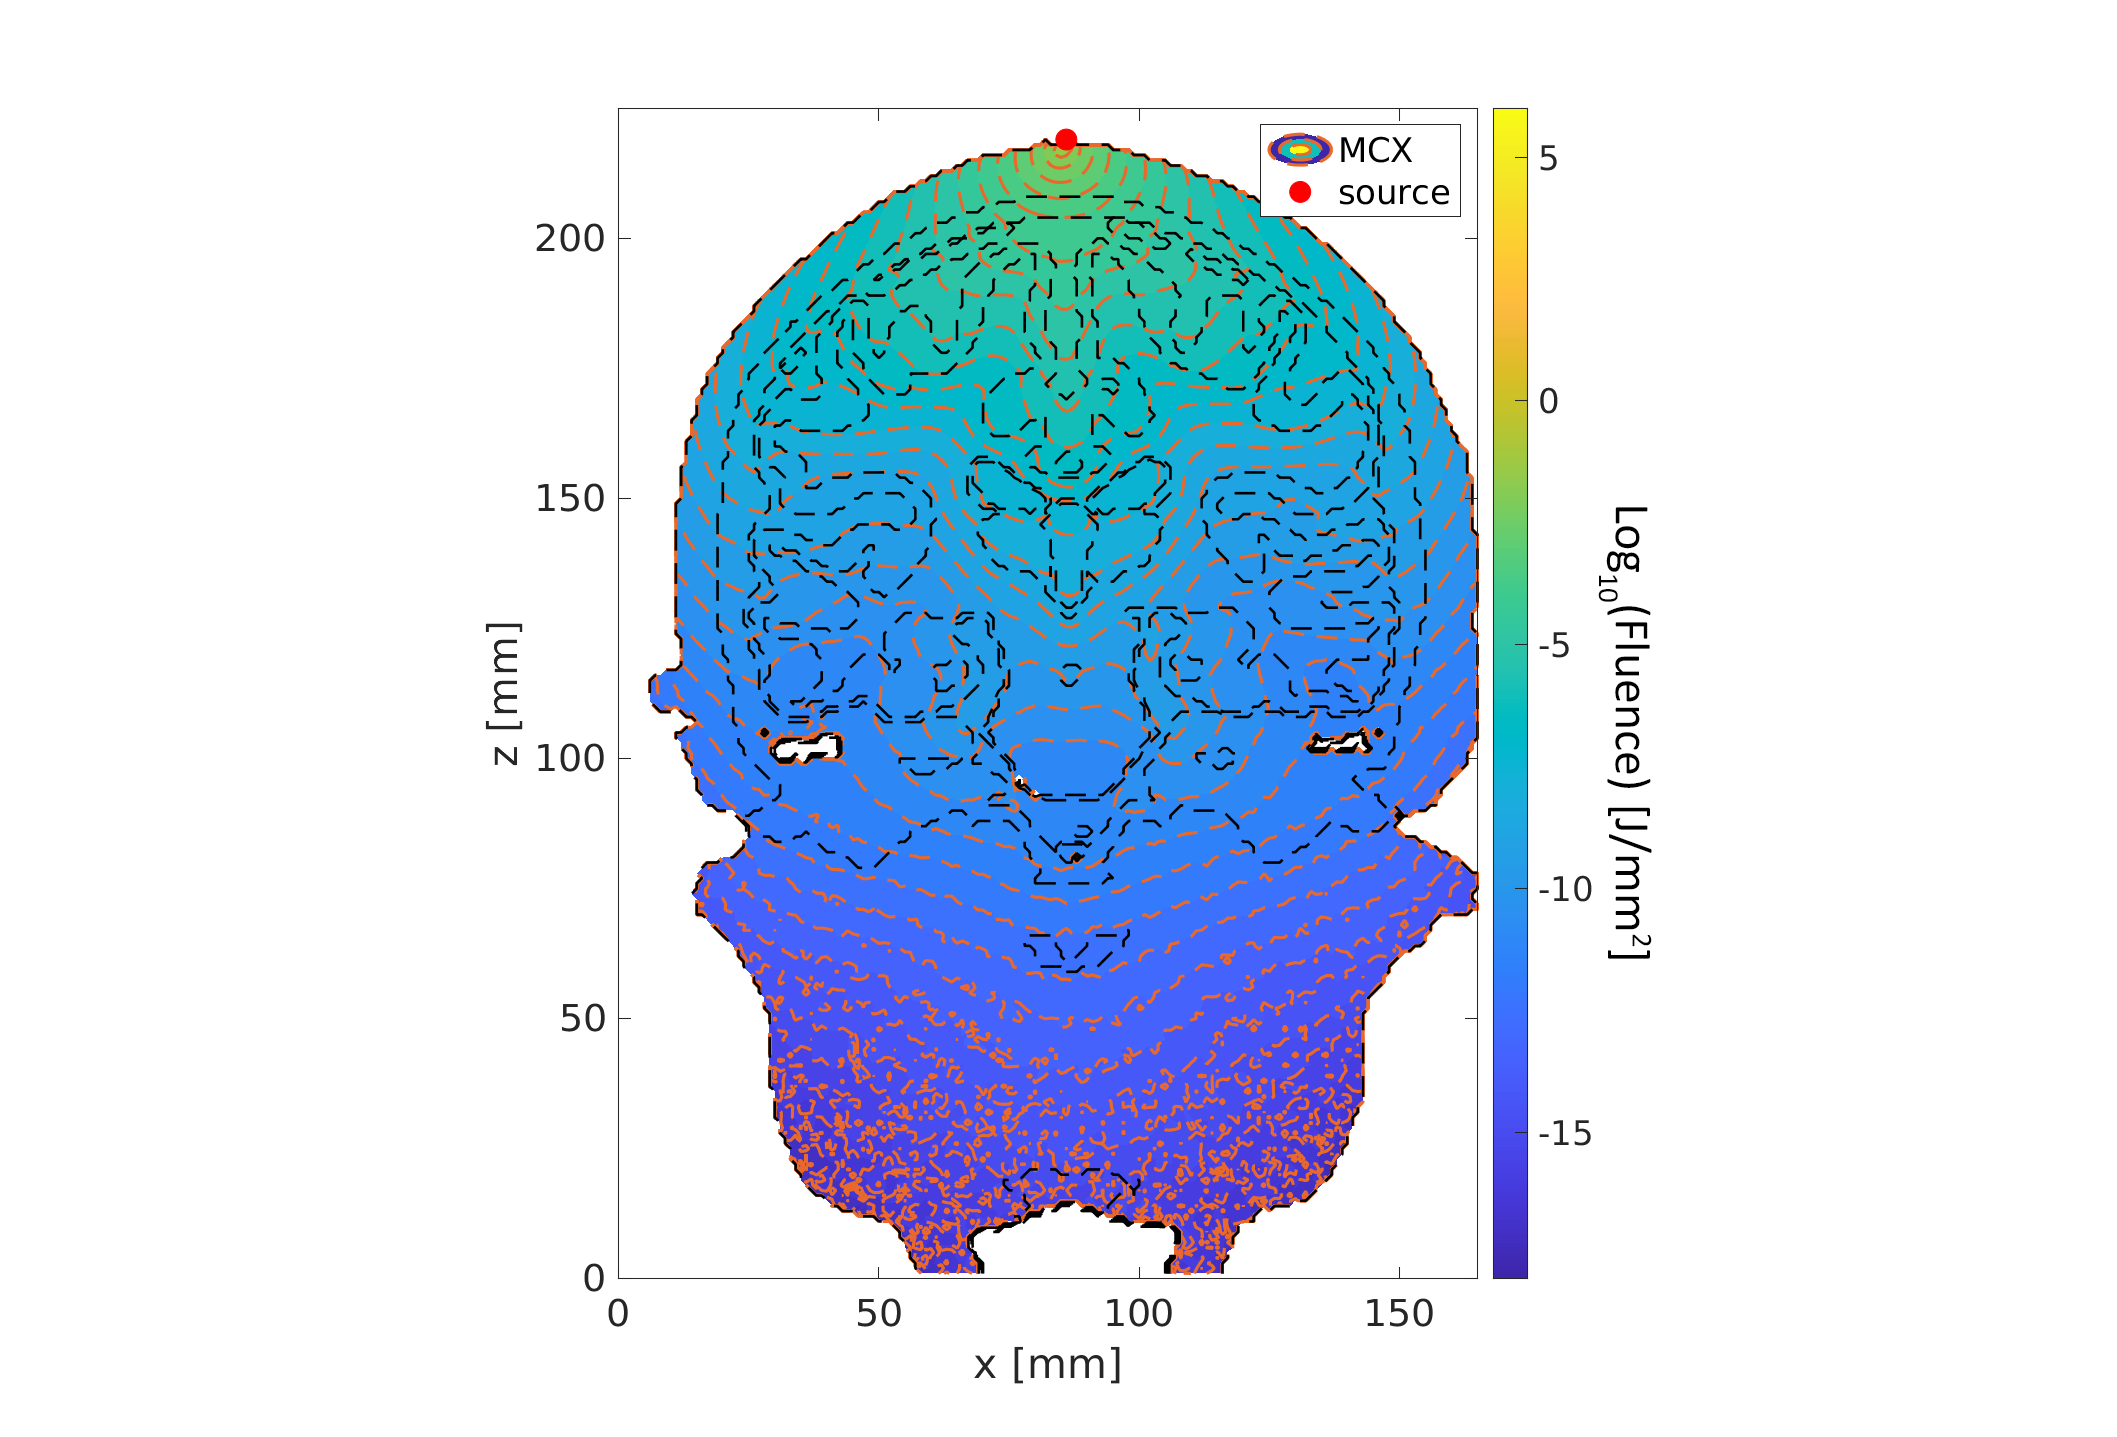
\includegraphics[width=\columnwidth]
    {Figures/Fluence_Distribution_980nm_CZ.png}}
    \caption{\label{fig:980-CZ} 980 nm CZ Position}
\end{figure}

\begin{figure}[!htb]
    \center{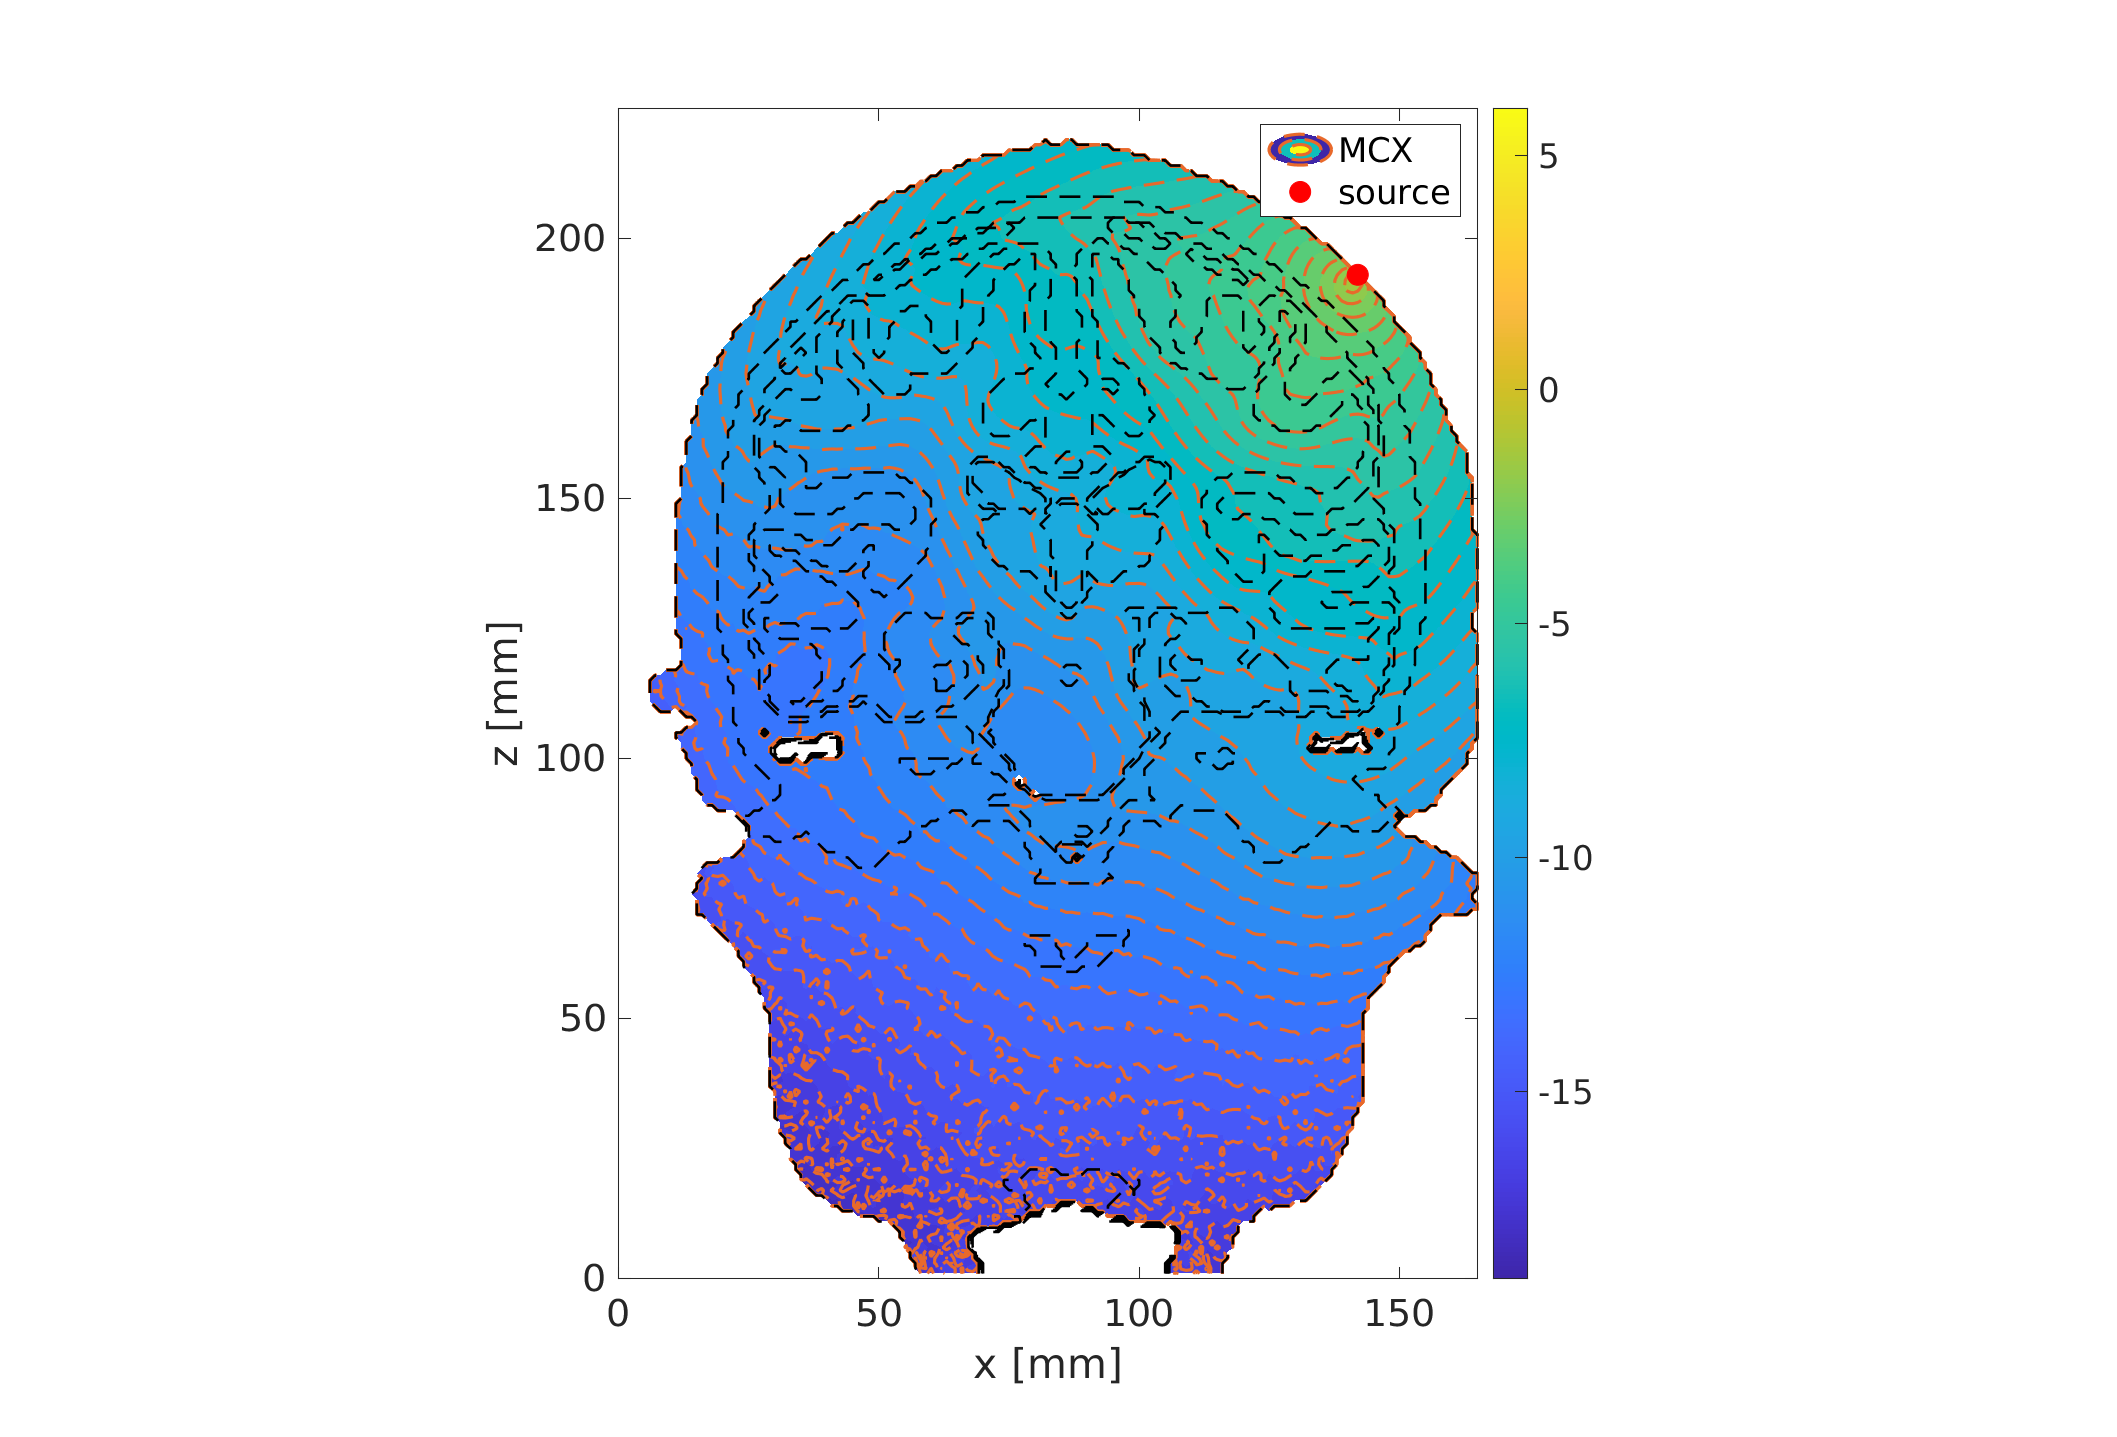
\includegraphics[width=\columnwidth]
    {Figures/Fluence_Distribution_980nm_45deg.png}}
    \caption{\label{fig:980-45} 980 nm 45 Degree Position}
\end{figure}

\begin{figure}[!htb]
    \center{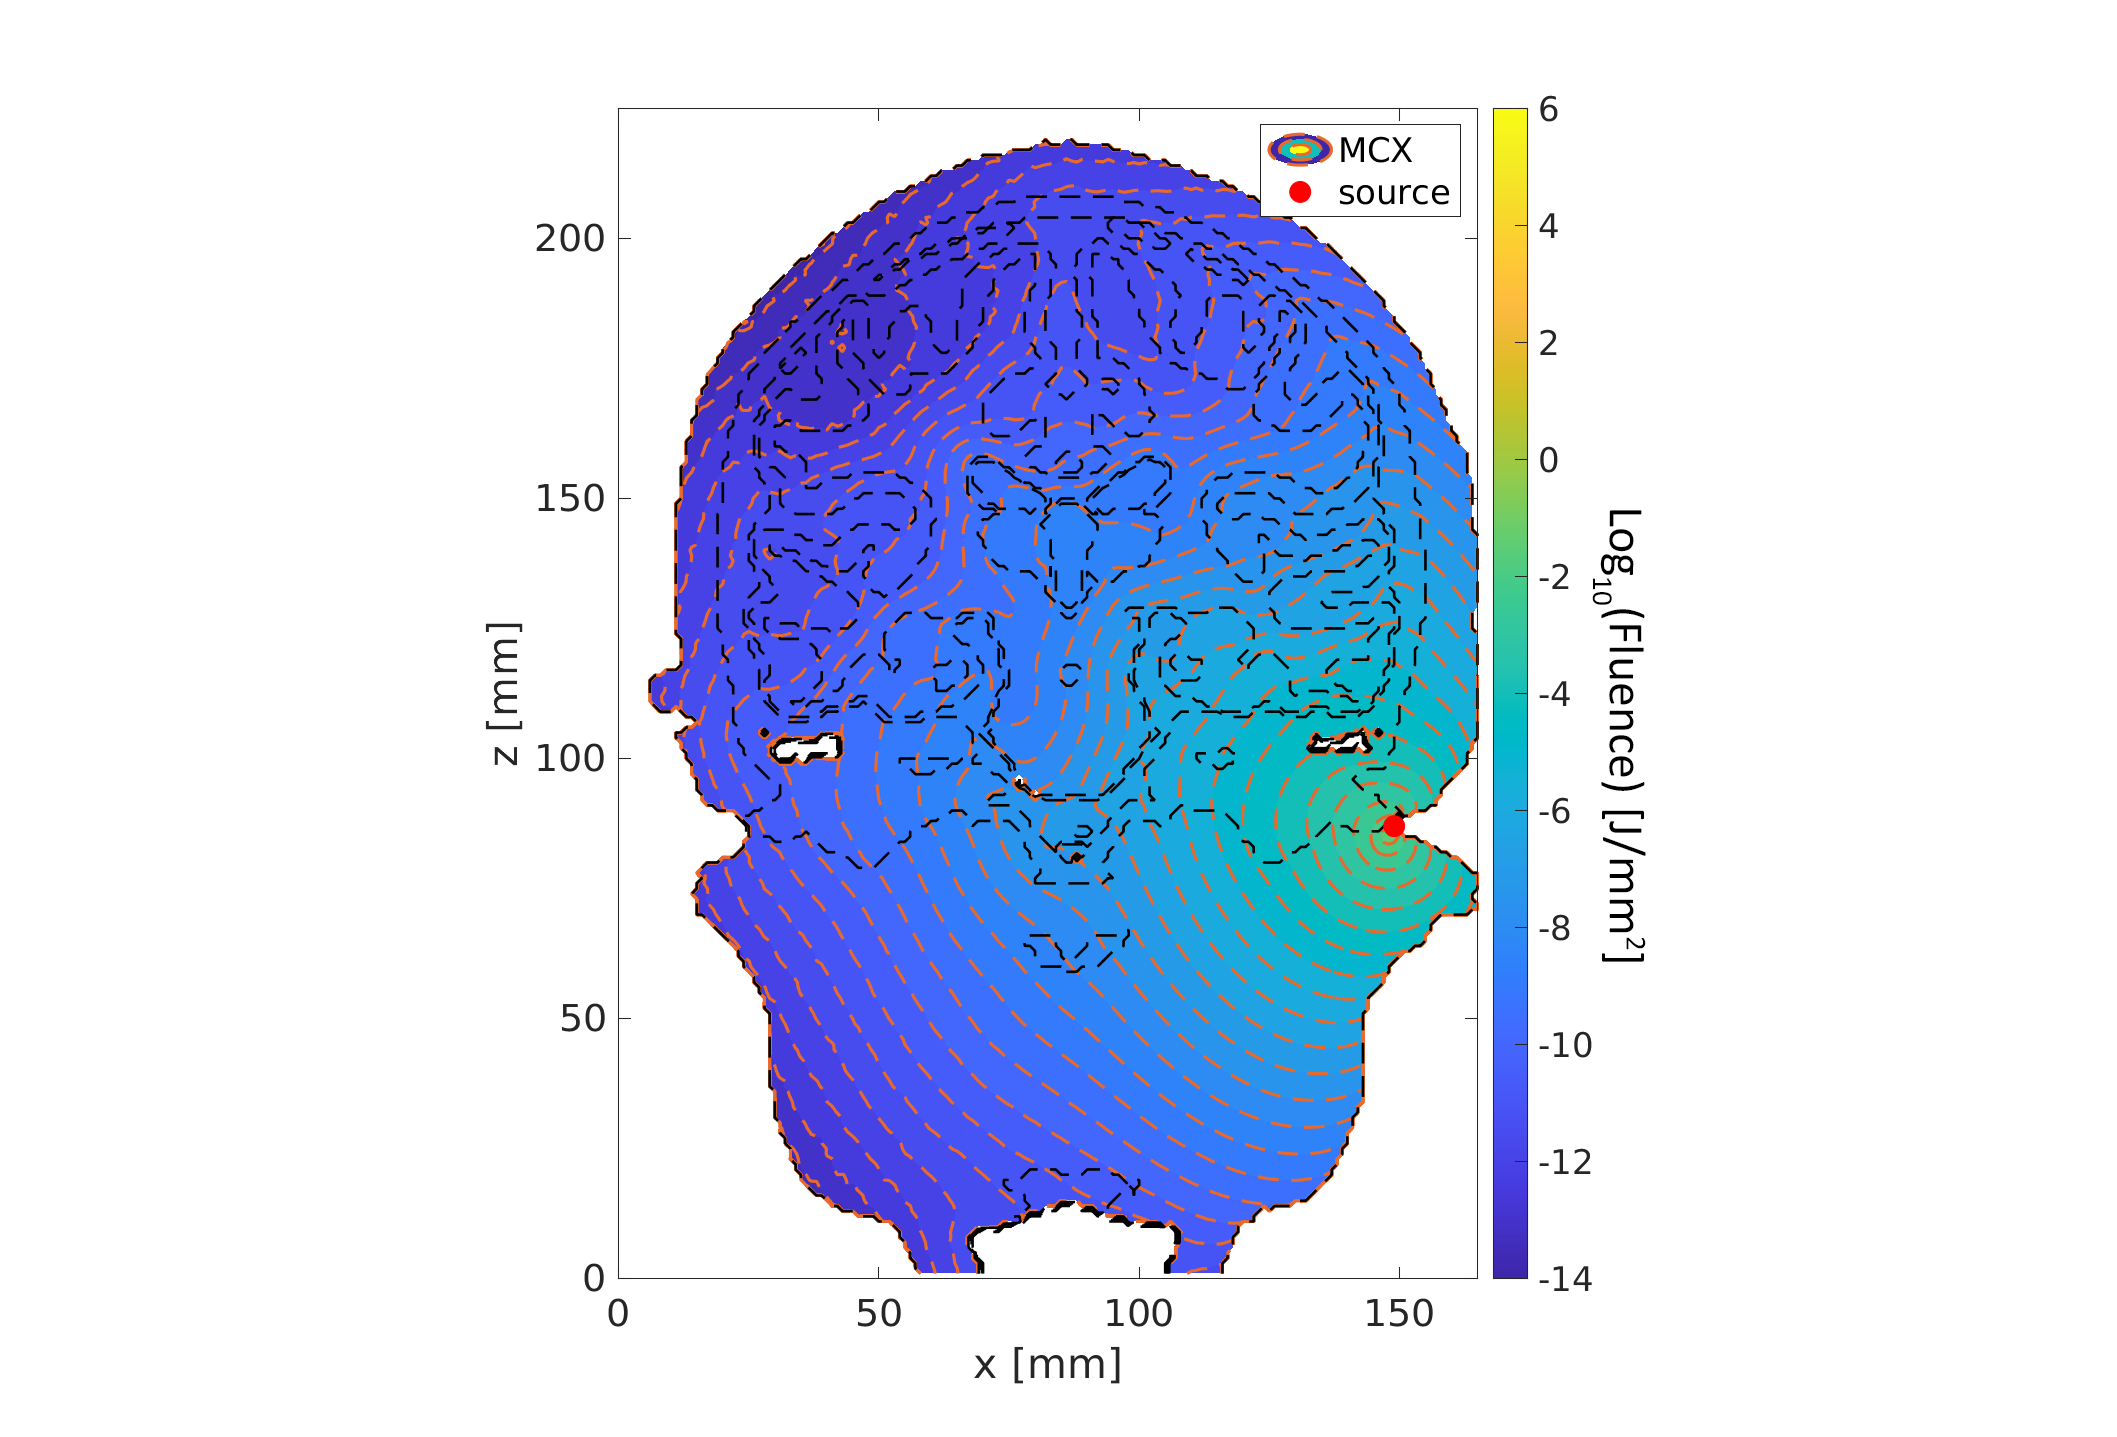
\includegraphics[width=\columnwidth]
    {Figures/Fluence_Distribution_980nm_Cochlear.png}}
    \caption{\label{fig:980-Cochlear} 980 nm Cochlear Position}
\end{figure}

\begin{figure}[!htb]
    \center{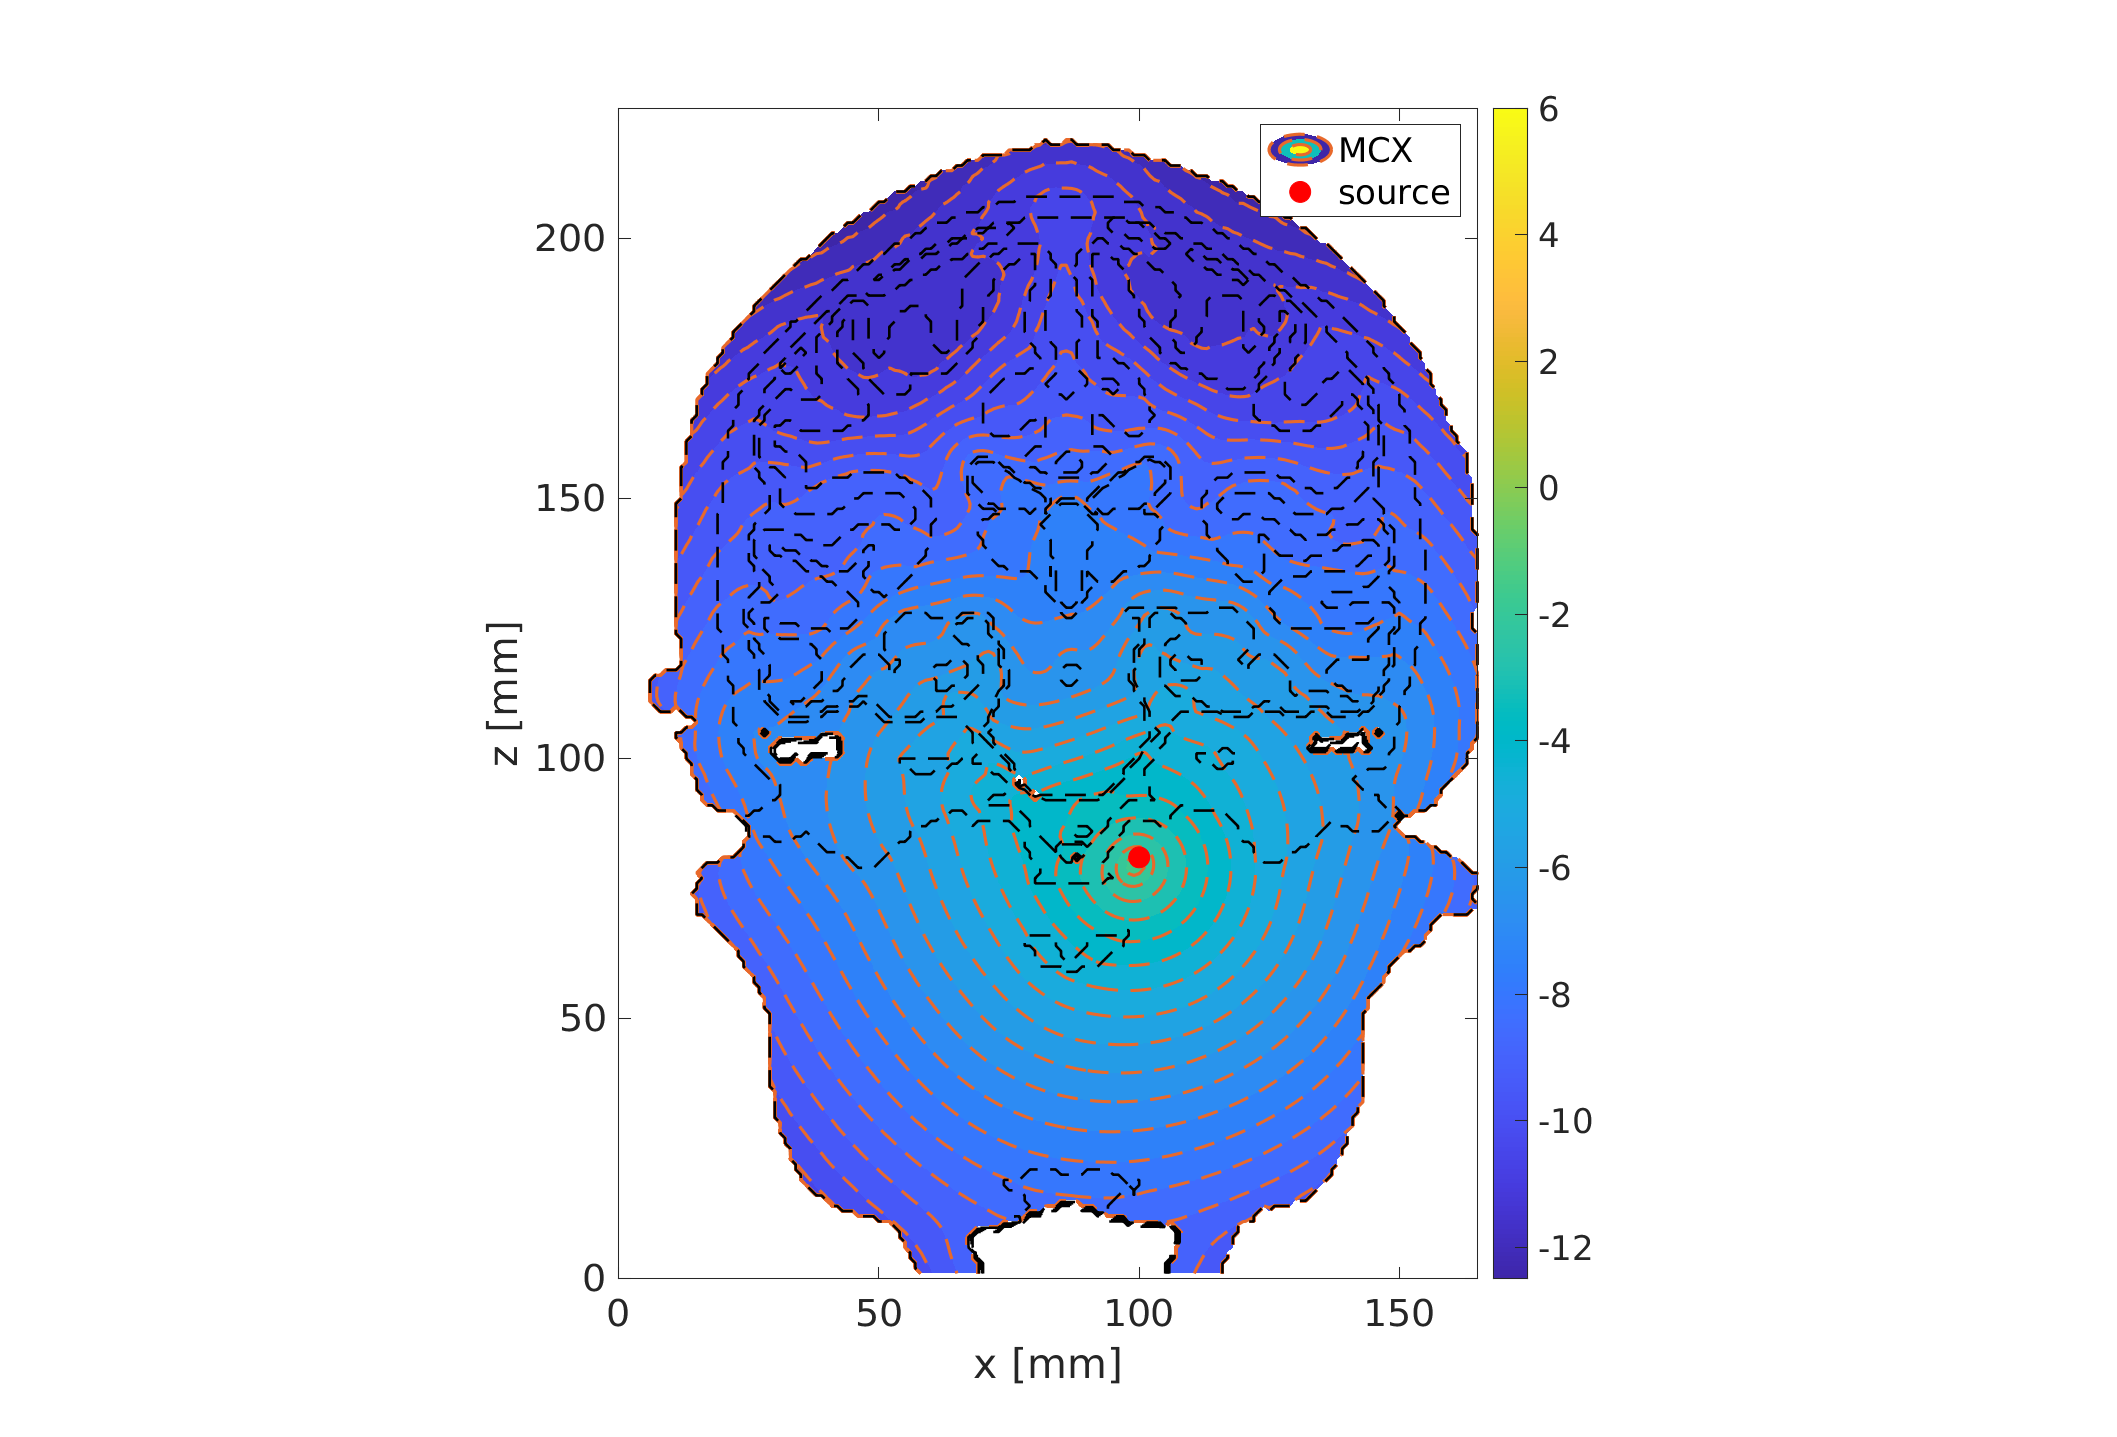
\includegraphics[width=\columnwidth]
    {Figures/Fluence_Distribution_980nm_Intranasal.png}}
    \caption{\label{fig:980-Intra} 980 nm Intranasal Position}
\end{figure}

\begin{figure}[!htb]
    \center{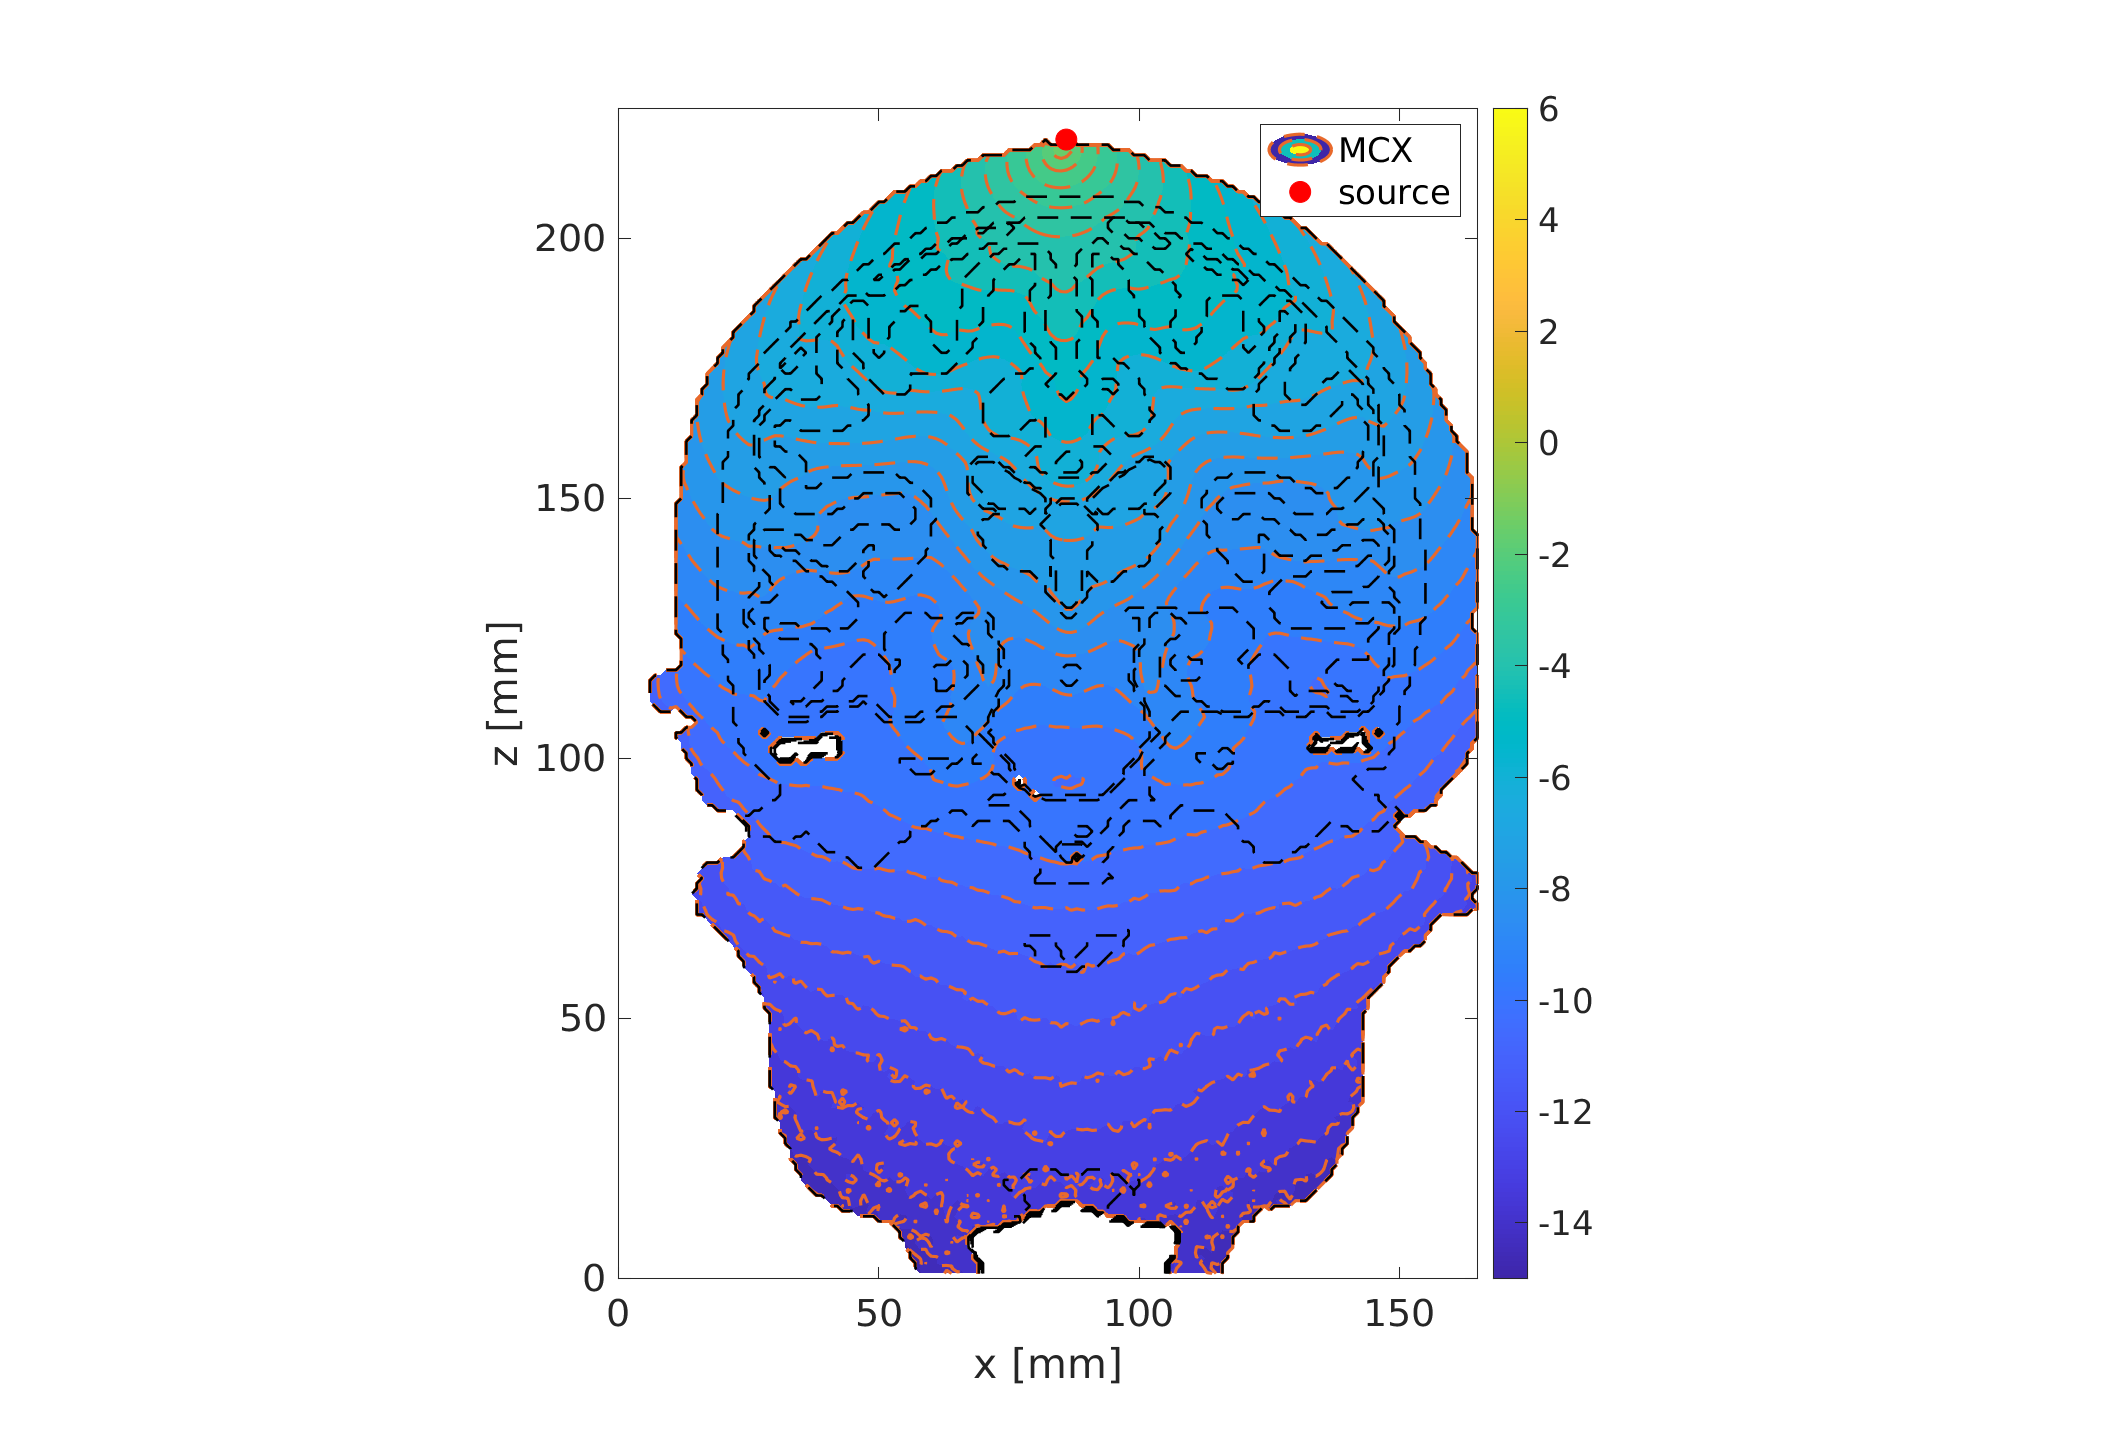
\includegraphics[width=\columnwidth]
    {Figures/Fluence_Distribution_1064nm_CZ.png}}
    \caption{\label{fig:1064-CZ} 1064 nm CZ Position}
\end{figure}

\begin{figure}[!htb]
    \center{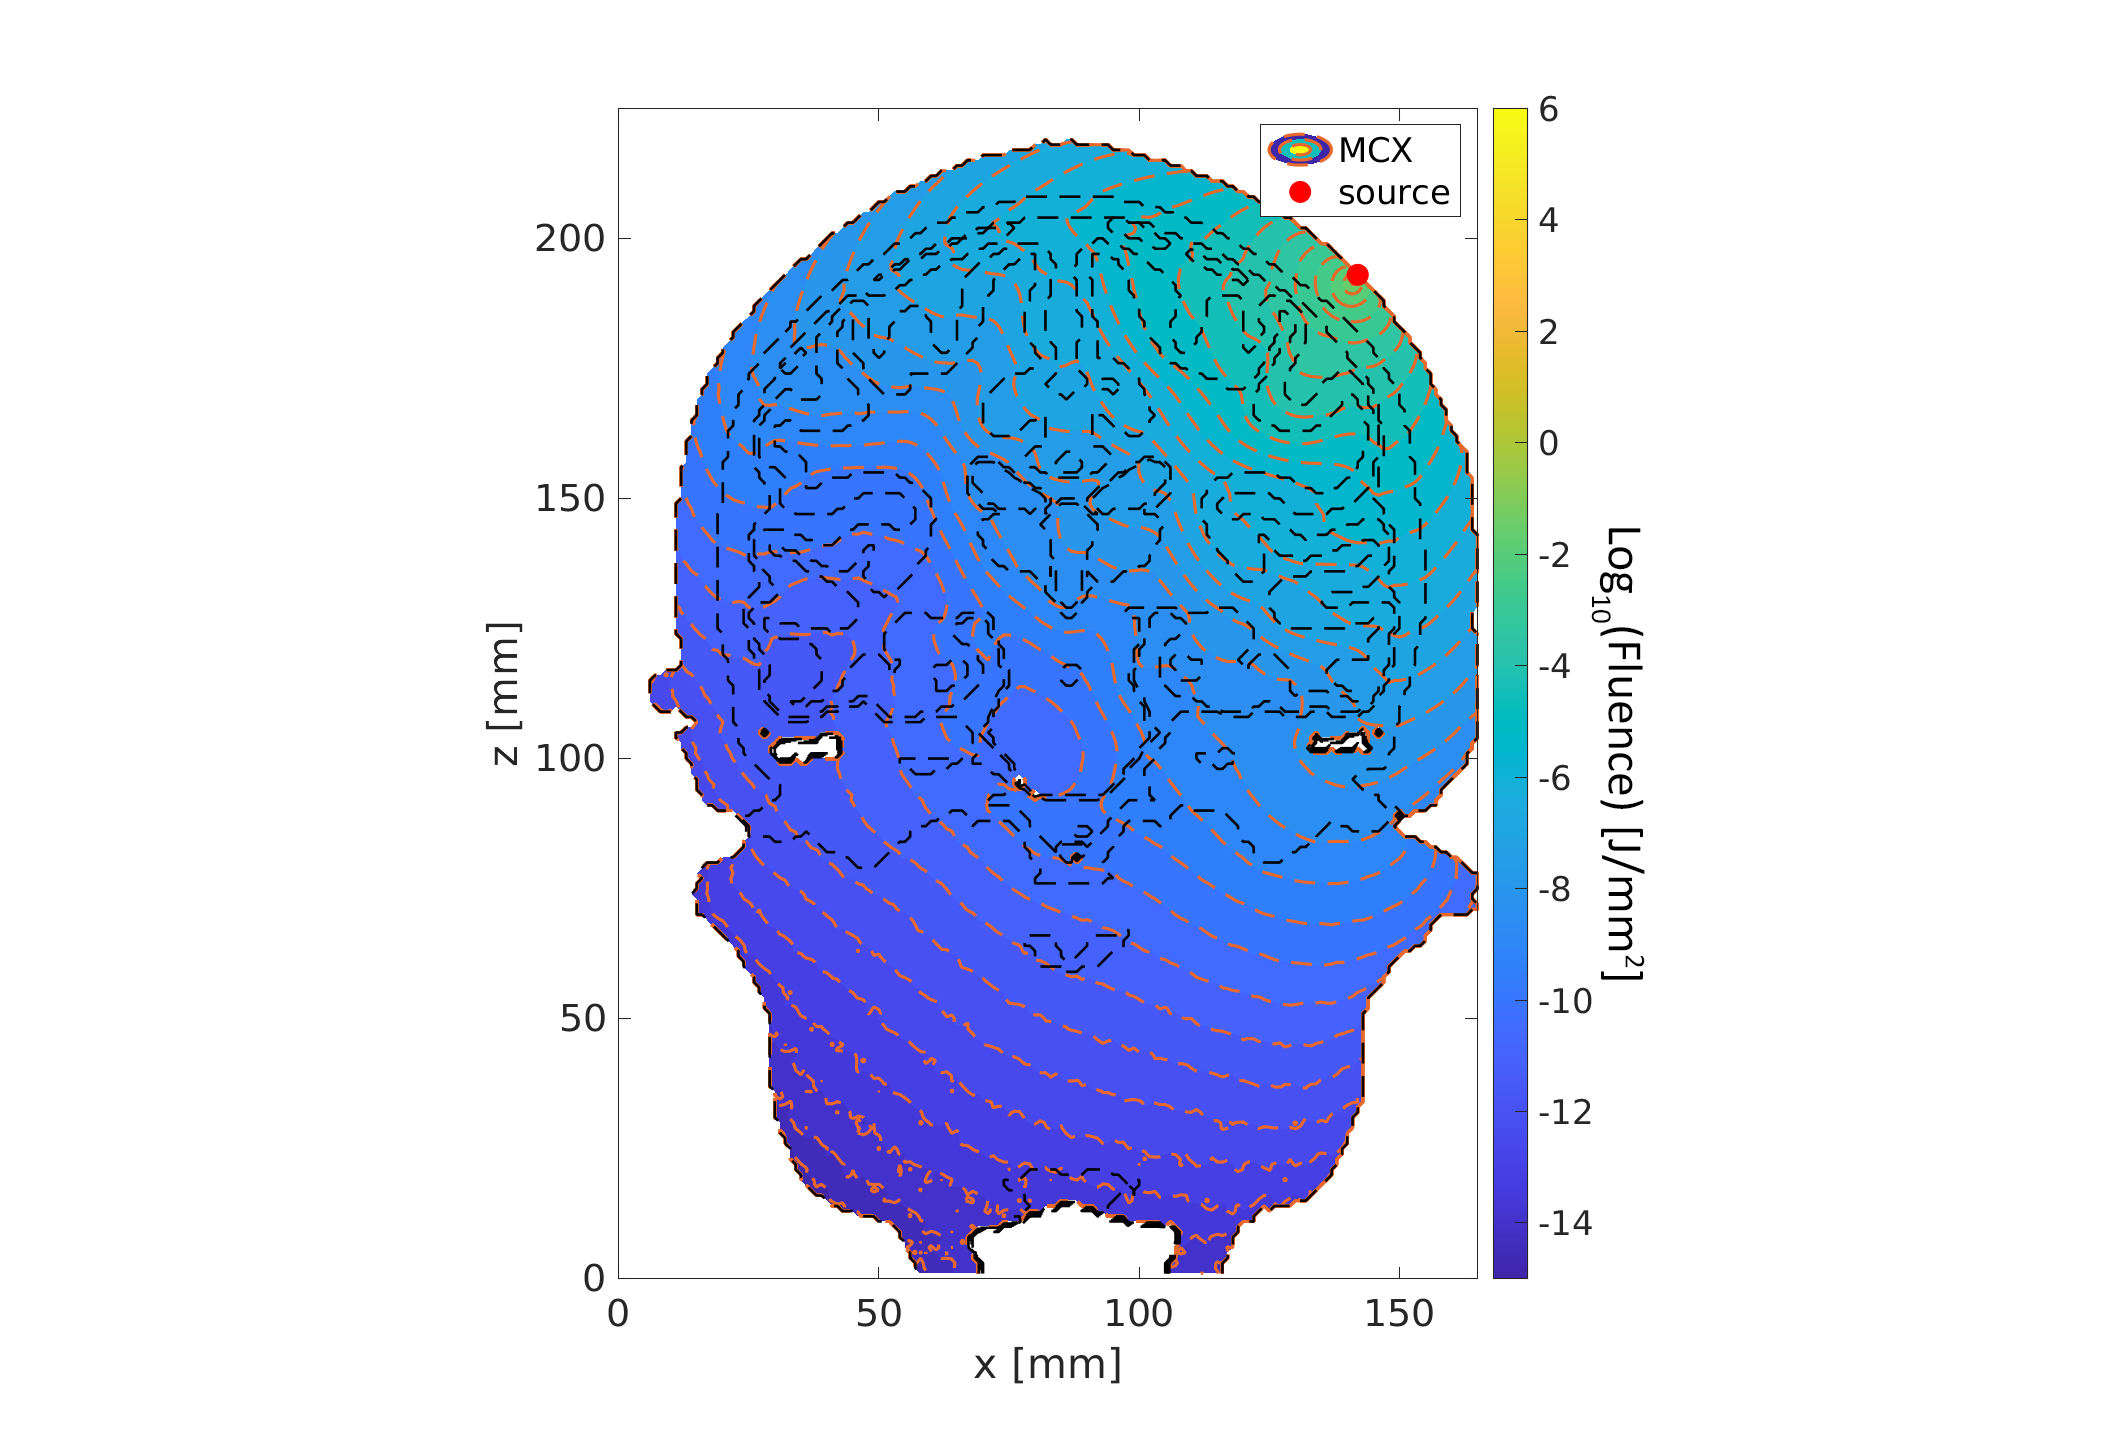
\includegraphics[width=\columnwidth]
    {Figures/Fluence_Distribution_1064nm_45deg.png}}
    \caption{\label{fig:1064-45} 1064 nm 45 Degree Position}
\end{figure}

\begin{figure}[!htb]
    \center{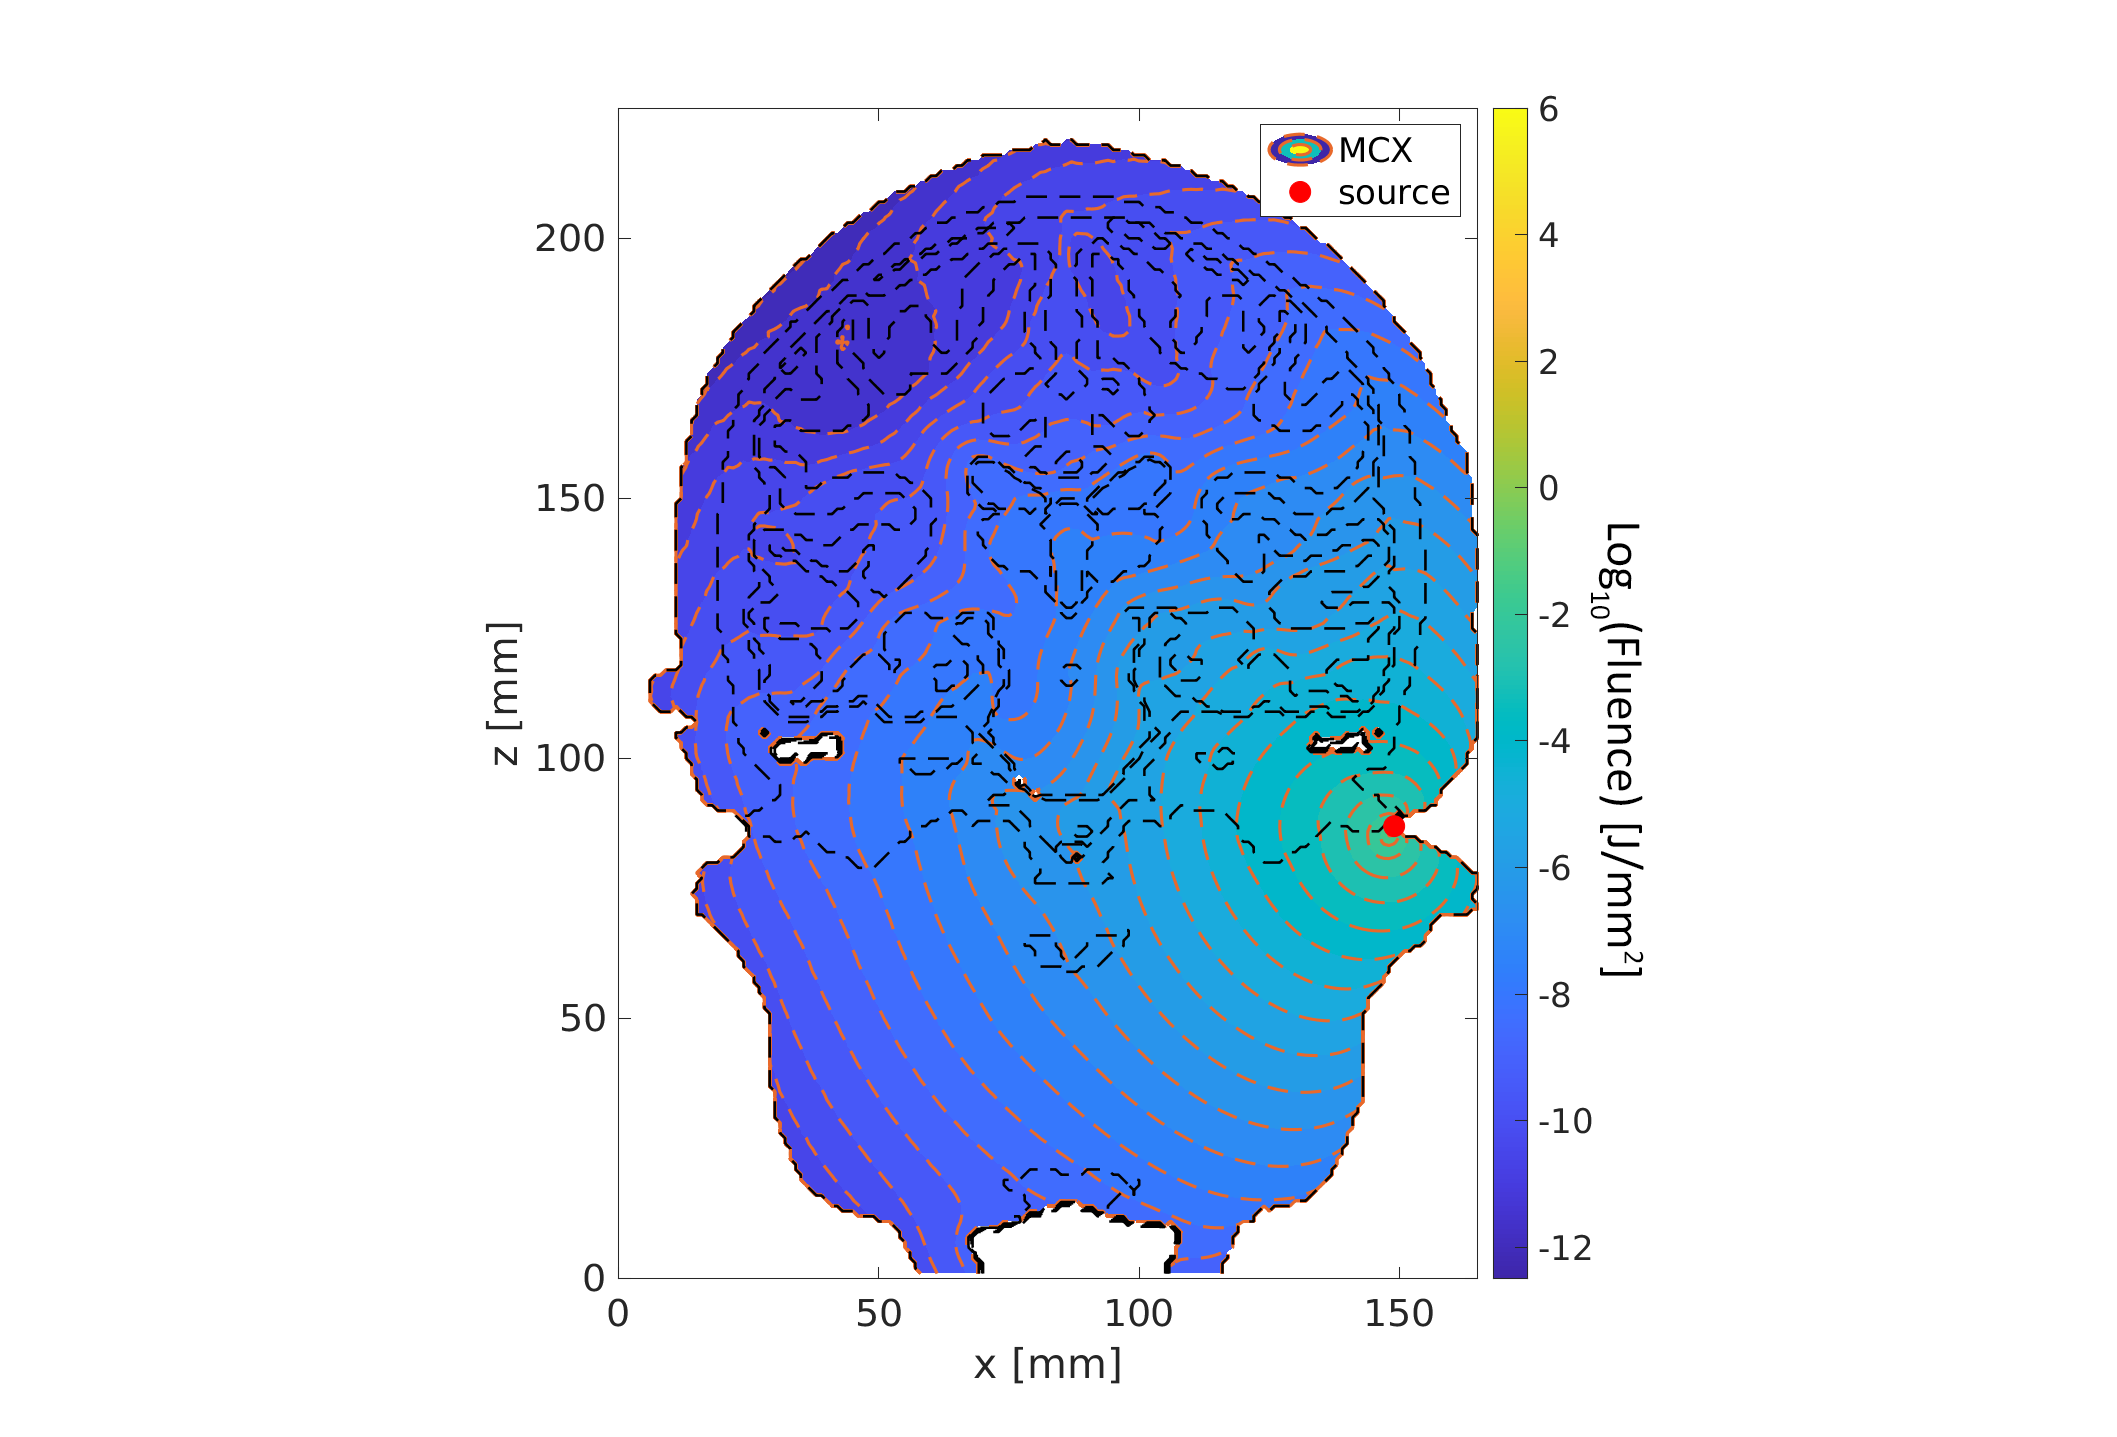
\includegraphics[width=\columnwidth]
    {Figures/Fluence_Distribution_1064nm_Cochlear.png}}
    \caption{\label{fig:1064-Cochlear} 1064 nm Cochlear Position}
\end{figure}

\begin{figure}[!htb]
    \center{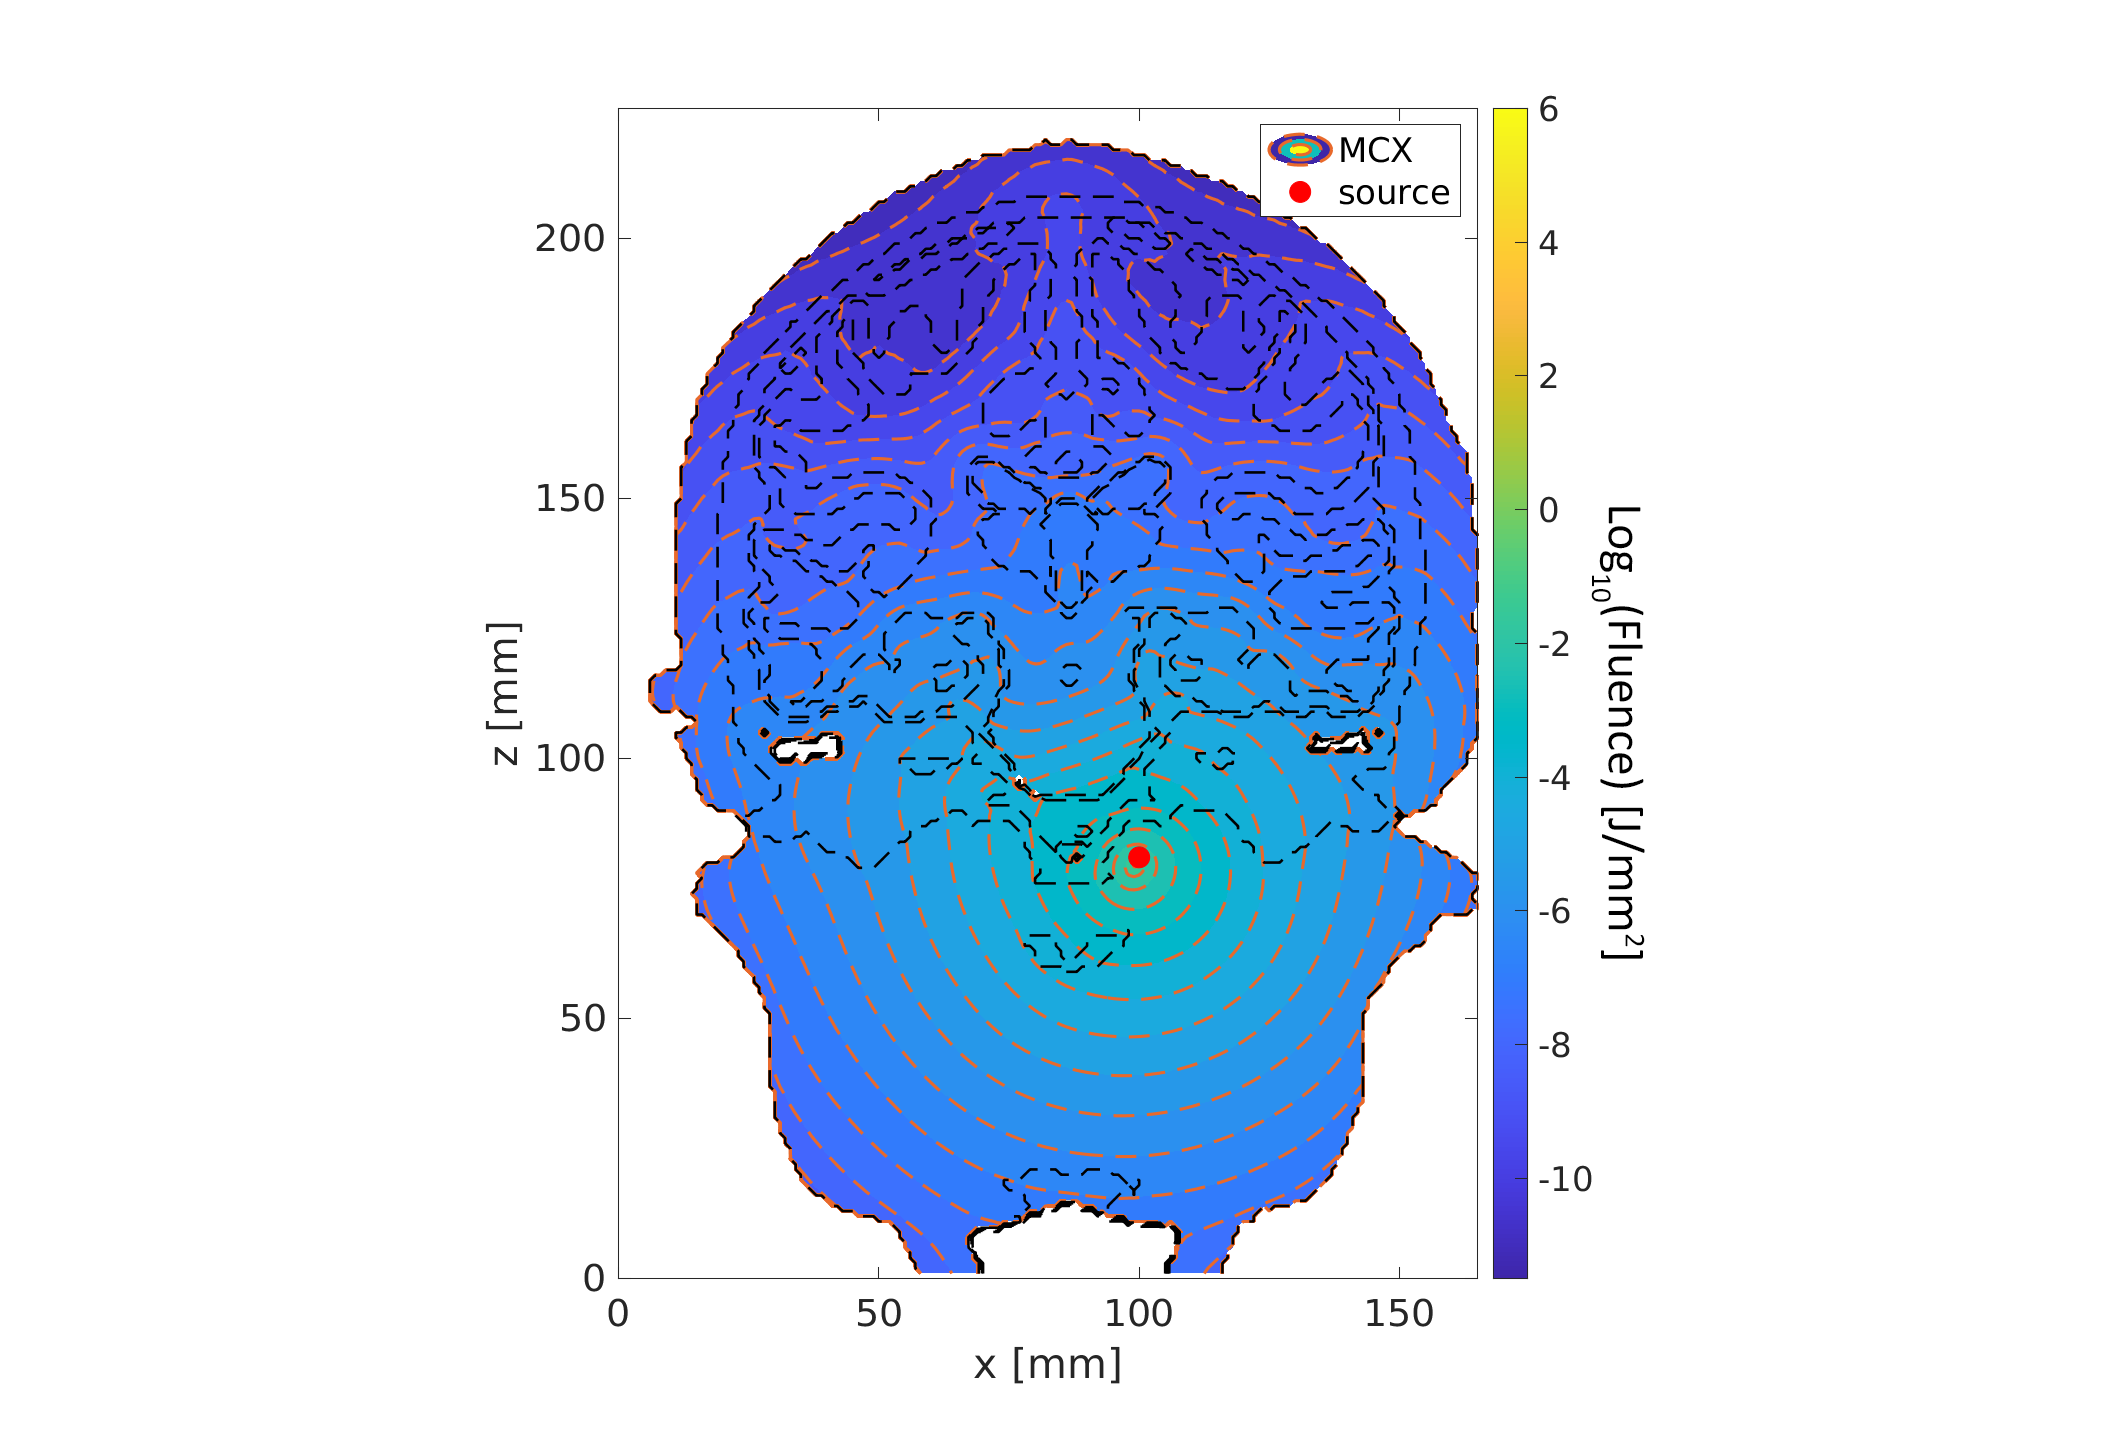
\includegraphics[width=\columnwidth]
    {Figures/Fluence_Distribution_1064nm_Intranasal.png}}
    \caption{\label{fig:1064-Intra} 1064 nm Intranasal Position}
\end{figure}

\begin{figure}[!htb]
    \center{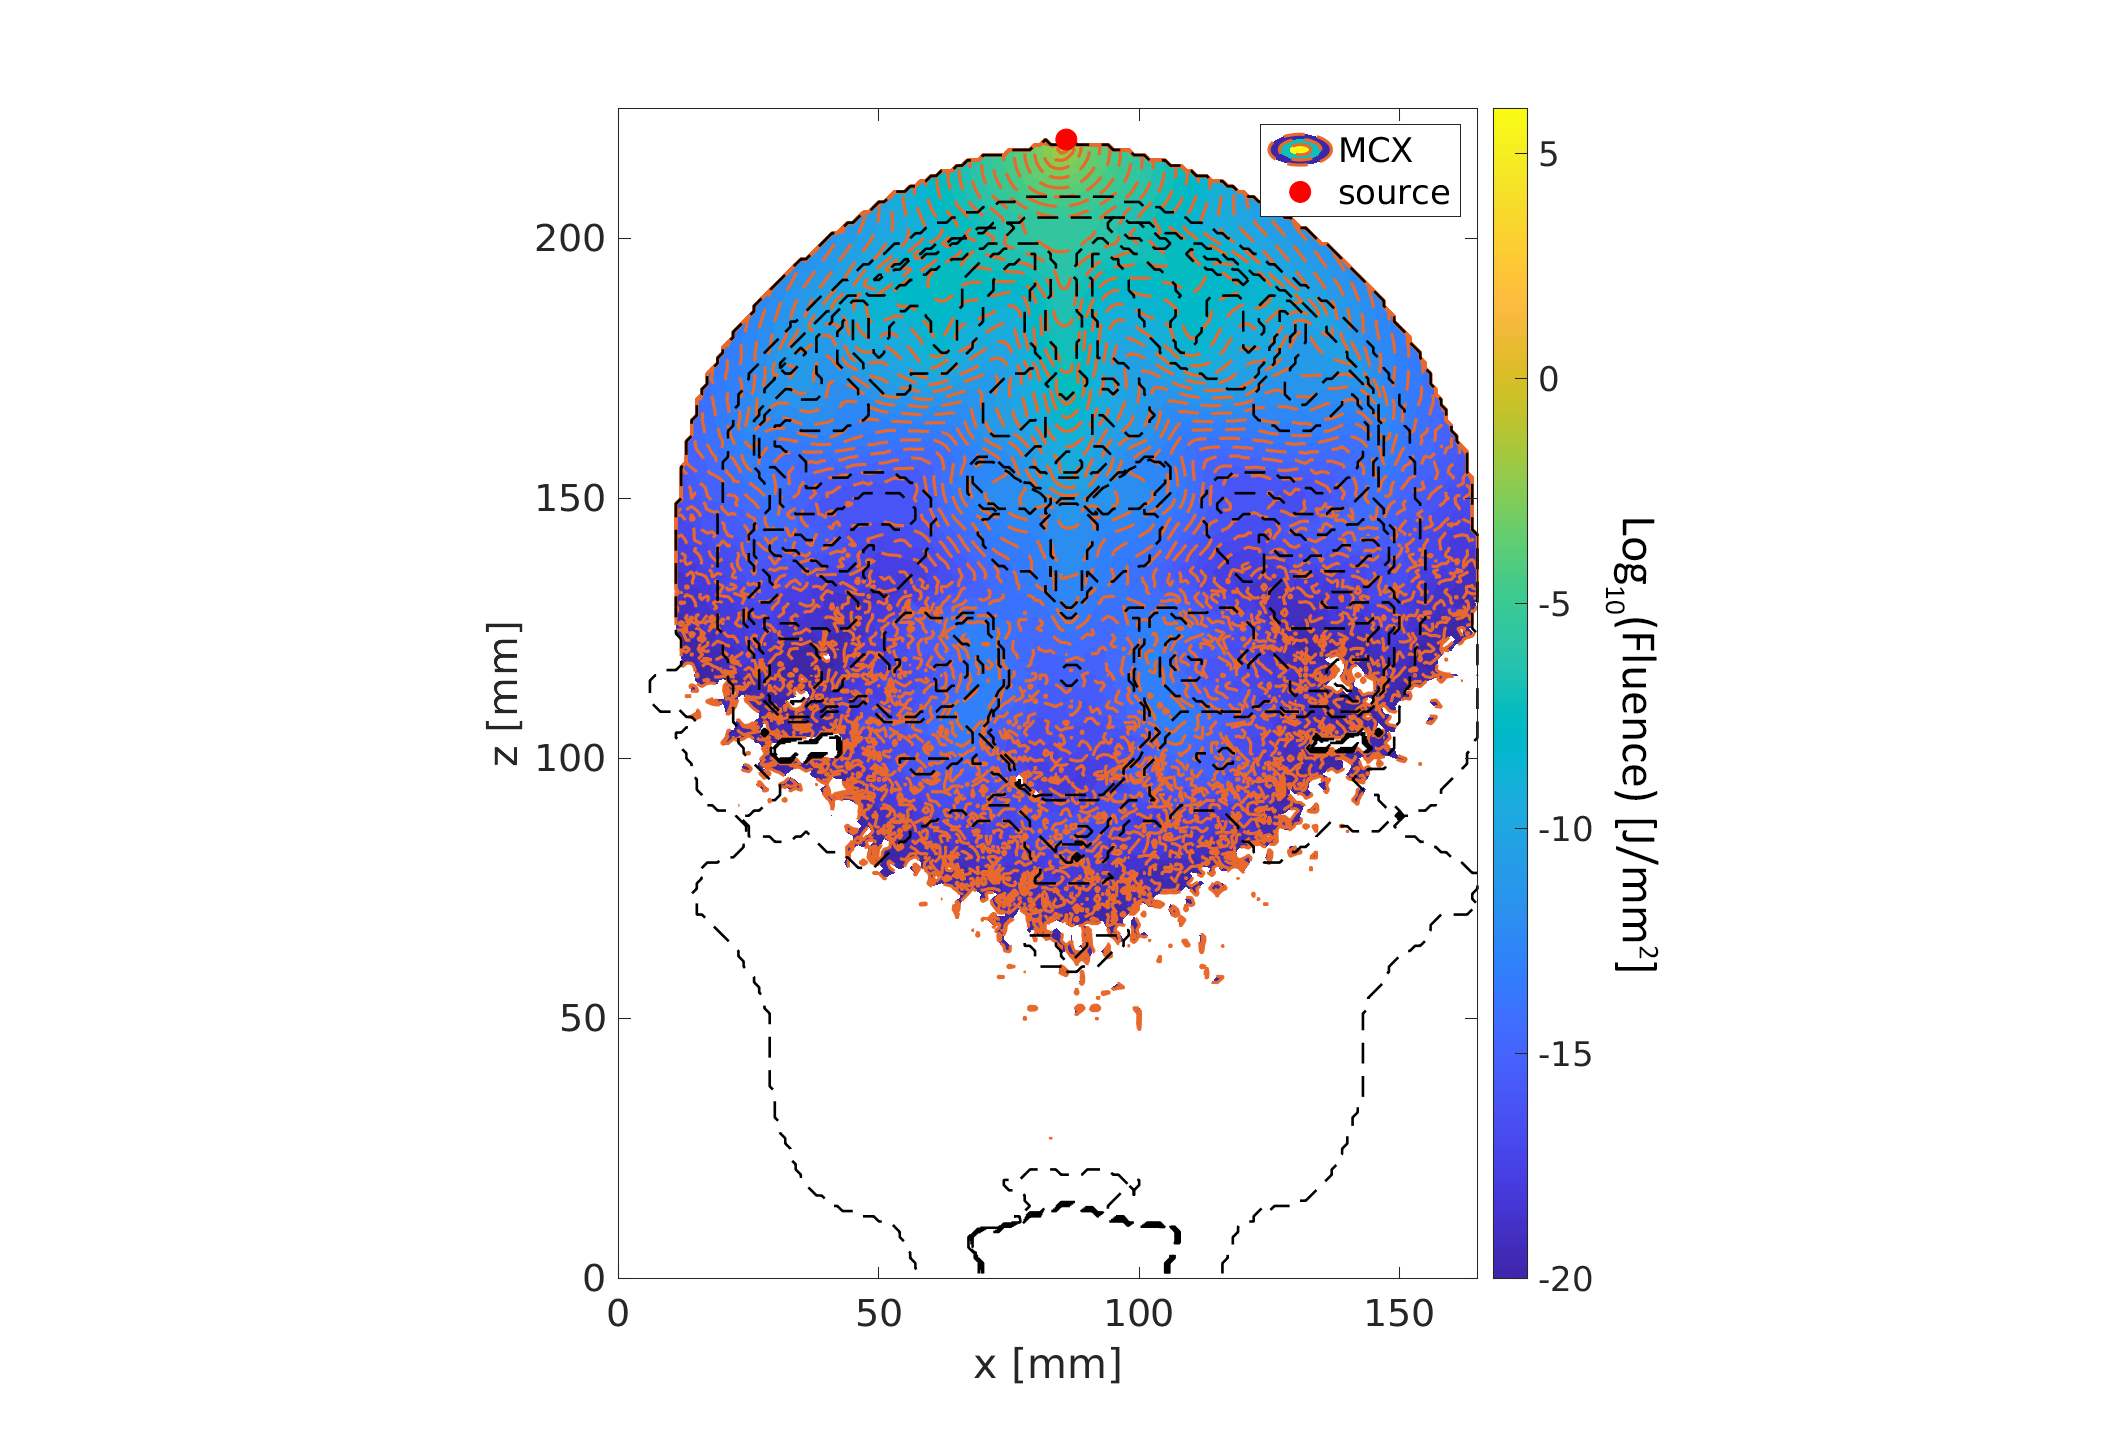
\includegraphics[width=\columnwidth]
    {Figures/Fluence_Distribution_1550nm_CZ.png}}
    \caption{\label{fig:1550-CZ} 1550 nm CZ Position}
\end{figure}

\begin{figure}[!htb]
    \center{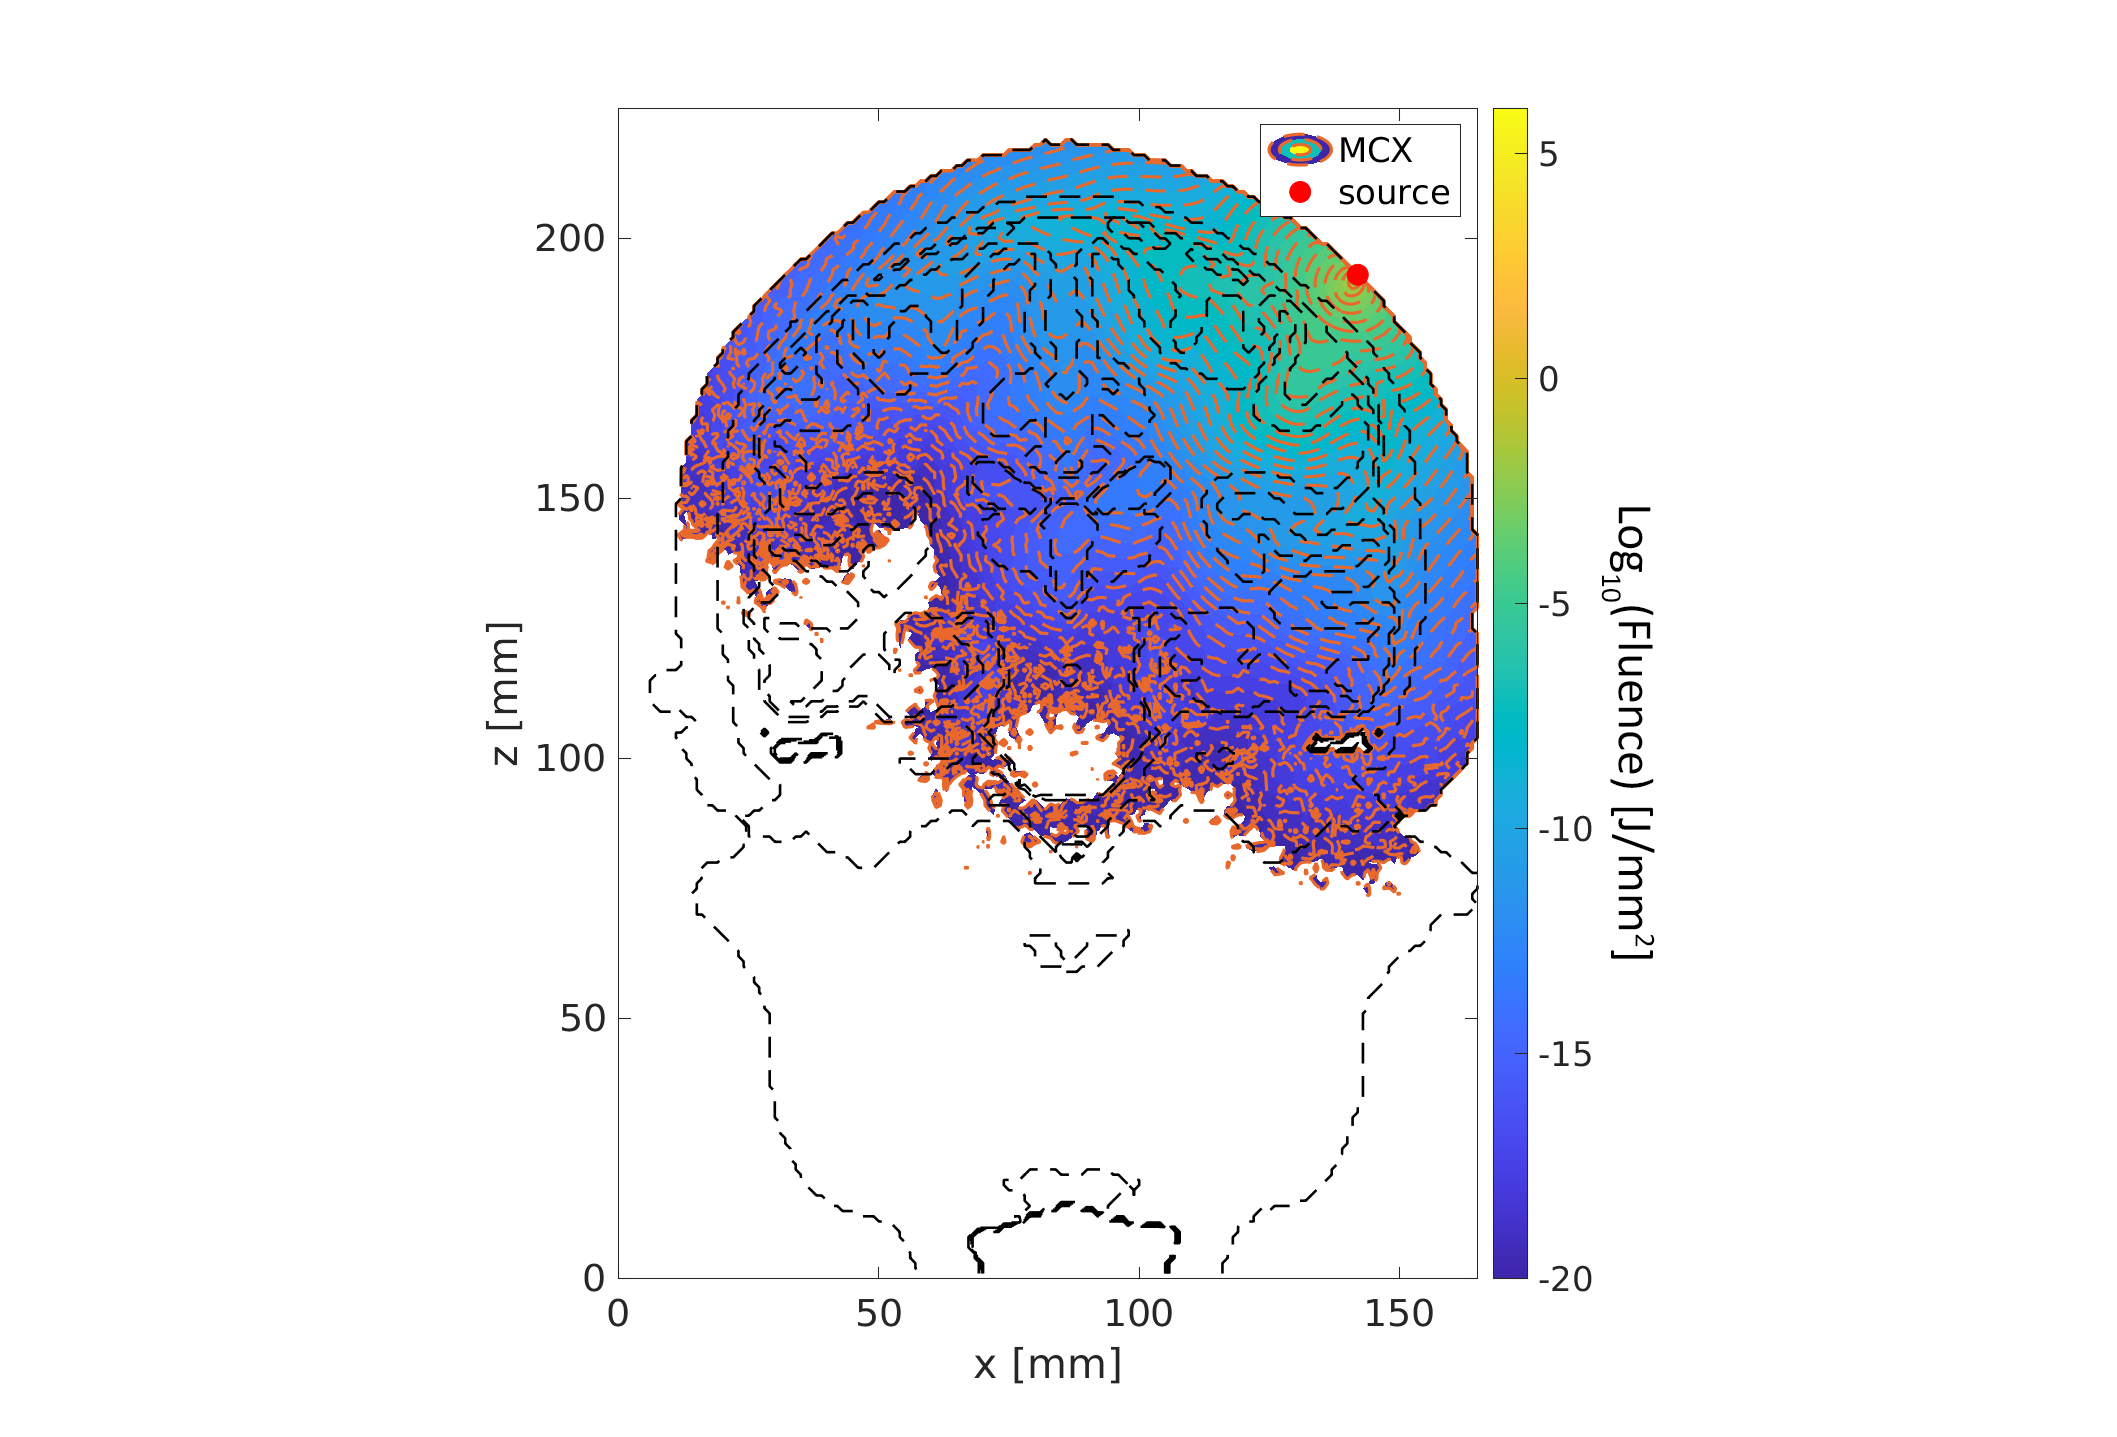
\includegraphics[width=\columnwidth]
    {Figures/Fluence_Distribution_1550nm_45deg.png}}
    \caption{\label{fig:1550-45} 1550 nm 45 Degree Position}
\end{figure}

\begin{figure}[!htb]
    \center{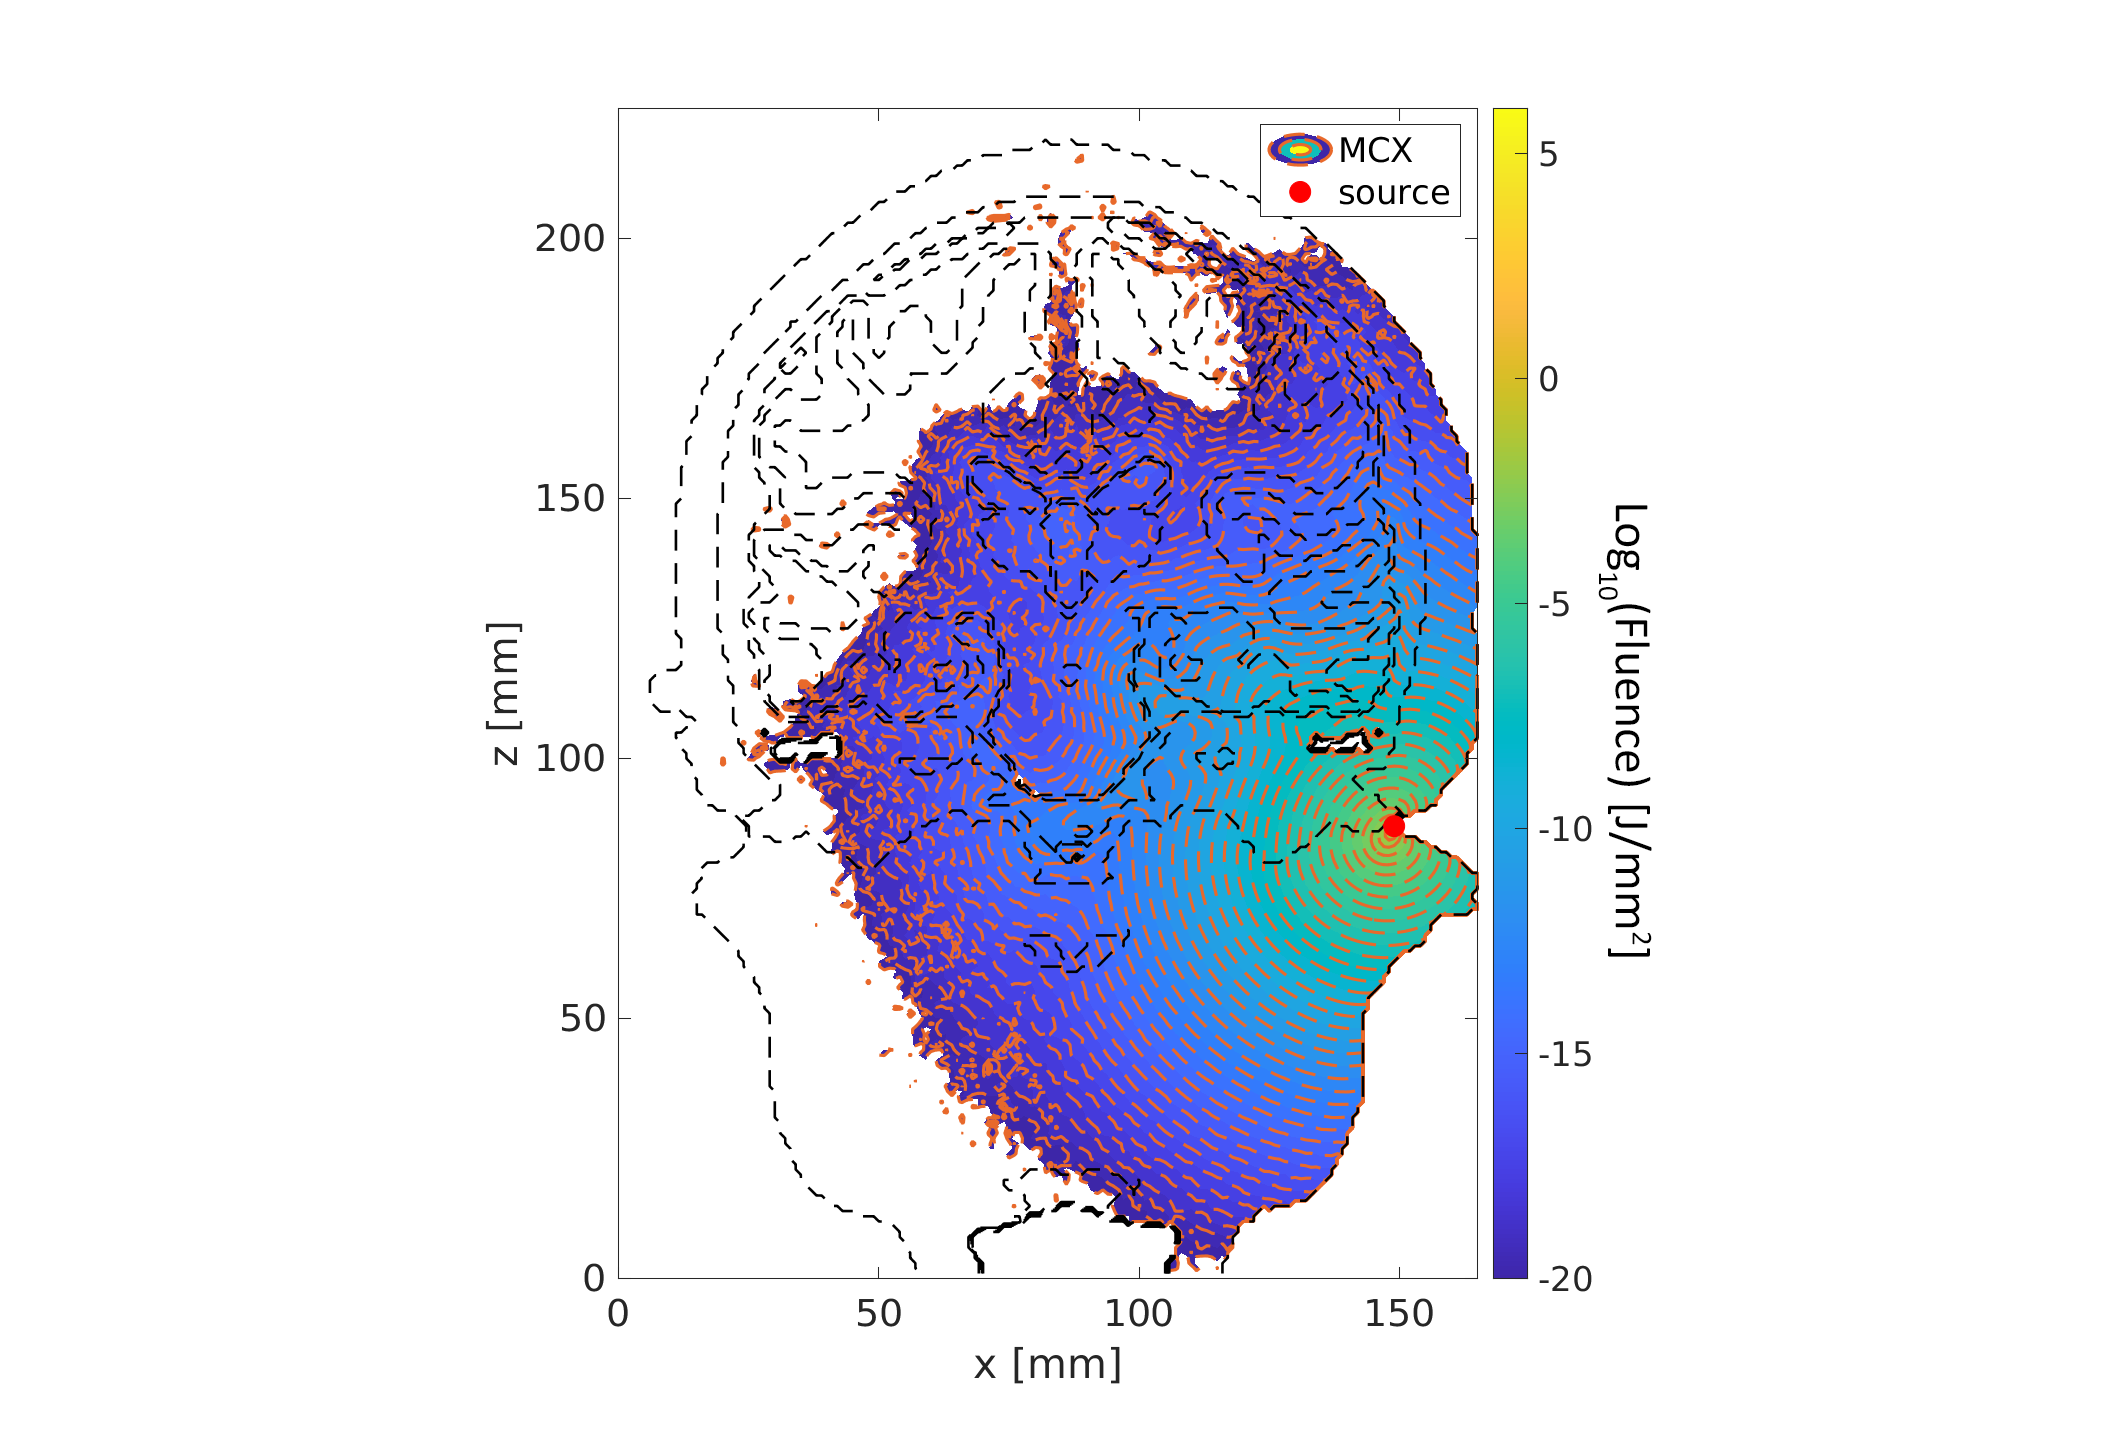
\includegraphics[width=\columnwidth]
    {Figures/Fluence_Distribution_1550nm_Cochlear.png}}
    \caption{\label{fig:1550-Cochlear} 1550 nm Cochlear Position}
\end{figure}

\begin{figure}[!htb]
    \center{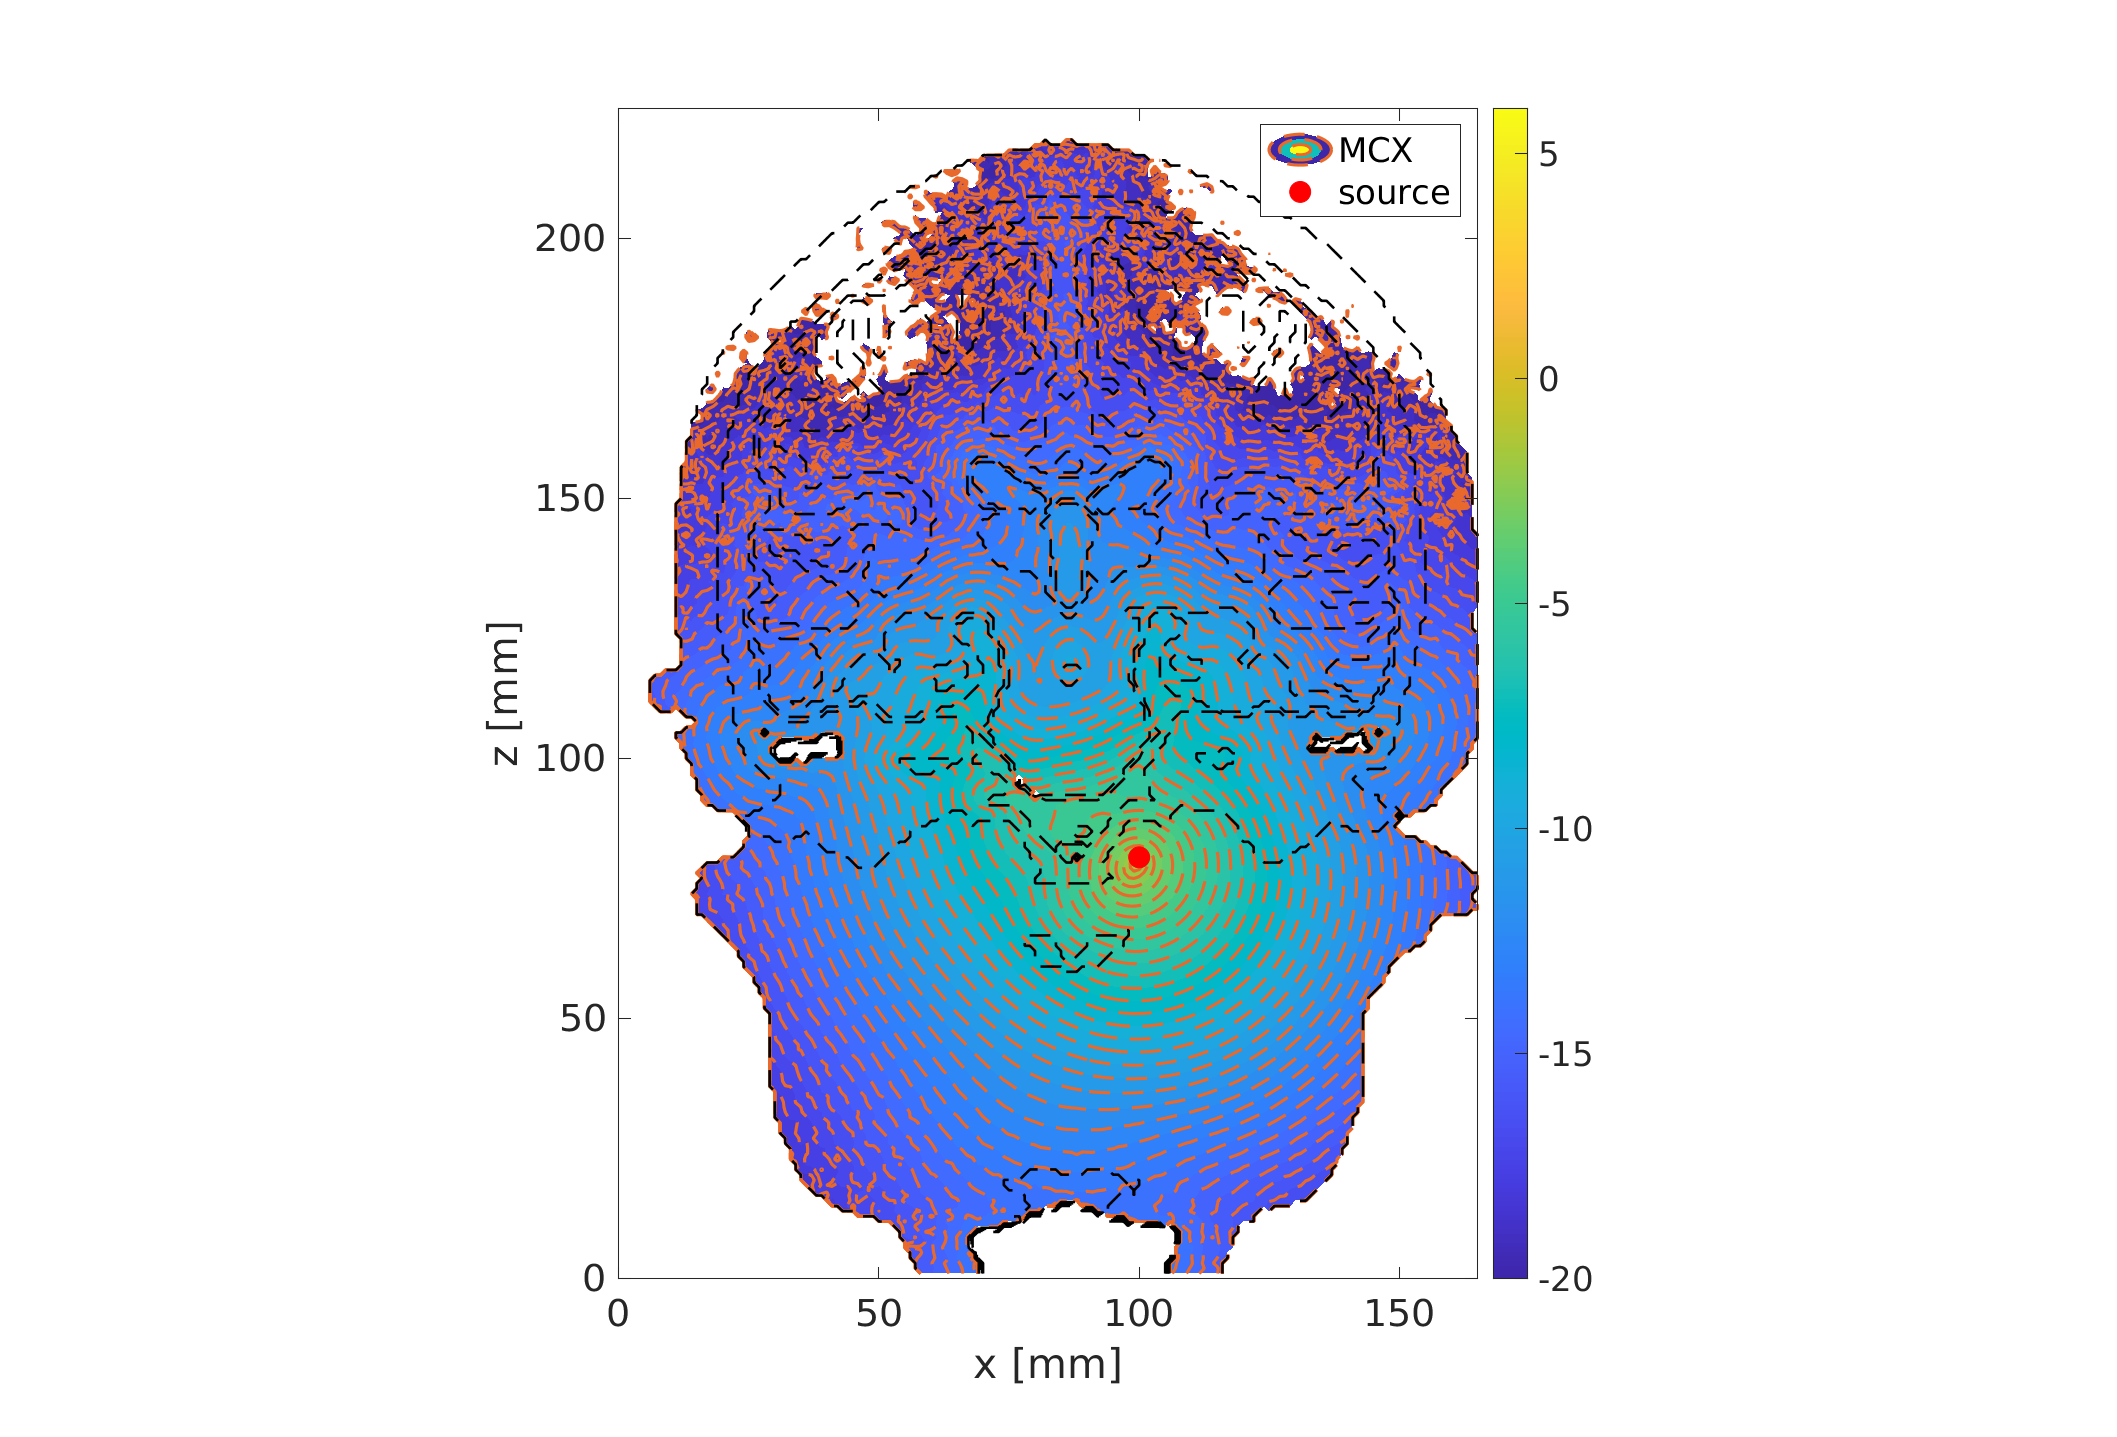
\includegraphics[width=\columnwidth]
    {Figures/Fluence_Distribution_1550nm_Intranasal.png}}
    \caption{\label{fig:1550-Intra} 1550 nm Intranasal Position}
\end{figure}

\section{Next Steps}
\label{sec:next steps}

\section{Conclusion}
\label{sec:conclusion}

\section*{Acknowledgment}

\section*{References}

\end{document}
